%  LaTeX support: latex@mdpi.com 
%  For support, please attach all files needed for compiling as well as the log file, and specify your operating system, LaTeX version, and LaTeX editor.

%=================================================================
\documentclass[remotesensing,article,submit,pdftex,moreauthors]{Definitions/mdpi}

%--------------------
% Class Options:
%--------------------
%----------
% journal
%----------
% Choose between the following MDPI journals:
% acoustics, actuators, addictions, admsci, adolescents, aerobiology, aerospace, agriculture, agriengineering, agrochemicals, agronomy, ai, air, algorithms, allergies, alloys, analytica, analytics, anatomia, animals, antibiotics, antibodies, antioxidants, applbiosci, appliedchem, appliedmath, applmech, applmicrobiol, applnano, applsci, aquacj, architecture, arm, arthropoda, arts, asc, asi, astronomy, atmosphere, atoms, audiolres, automation, axioms, bacteria, batteries, bdcc, behavsci, beverages, biochem, bioengineering, biologics, biology, biomass, biomechanics, biomed, biomedicines, biomedinformatics, biomimetics, biomolecules, biophysica, biosensors, biotech, birds, bloods, blsf, brainsci, breath, buildings, businesses, cancers, carbon, cardiogenetics, catalysts, cells, ceramics, challenges, chemengineering, chemistry, chemosensors, chemproc, children, chips, cimb, civileng, cleantechnol, climate, clinpract, clockssleep, cmd, coasts, coatings, colloids, colorants, commodities, compounds, computation, computers, condensedmatter, conservation, constrmater, cosmetics, covid, crops, cryptography, crystals, csmf, ctn, curroncol, cyber, dairy, data, ddc, dentistry, dermato, dermatopathology, designs, devices, diabetology, diagnostics, dietetics, digital, disabilities, diseases, diversity, dna, drones, dynamics, earth, ebj, ecologies, econometrics, economies, education, ejihpe, electricity, electrochem, electronicmat, electronics, encyclopedia, endocrines, energies, eng, engproc, entomology, entropy, environments, environsciproc, epidemiologia, epigenomes, est, fermentation, fibers, fintech, fire, fishes, fluids, foods, forecasting, forensicsci, forests, foundations, fractalfract, fuels, future, futureinternet, futurepharmacol, futurephys, futuretransp, galaxies, games, gases, gastroent, gastrointestdisord, gels, genealogy, genes, geographies, geohazards, geomatics, geosciences, geotechnics, geriatrics, grasses, gucdd, hazardousmatters, healthcare, hearts, hemato, hematolrep, heritage, higheredu, highthroughput, histories, horticulturae, hospitals, humanities, humans, hydrobiology, hydrogen, hydrology, hygiene, idr, ijerph, ijfs, ijgi, ijms, ijns, ijpb, ijtm, ijtpp, ime, immuno, informatics, information, infrastructures, inorganics, insects, instruments, inventions, iot, j, jal, jcdd, jcm, jcp, jcs, jcto, jdb, jeta, jfb, jfmk, jimaging, jintelligence, jlpea, jmmp, jmp, jmse, jne, jnt, jof, joitmc, jor, journalmedia, jox, jpm, jrfm, jsan, jtaer, jvd, jzbg, kidneydial, kinasesphosphatases, knowledge, land, languages, laws, life, liquids, literature, livers, logics, logistics, lubricants, lymphatics, machines, macromol, magnetism, magnetochemistry, make, marinedrugs, materials, materproc, mathematics, mca, measurements, medicina, medicines, medsci, membranes, merits, metabolites, metals, meteorology, methane, metrology, micro, microarrays, microbiolres, micromachines, microorganisms, microplastics, minerals, mining, modelling, molbank, molecules, mps, msf, mti, muscles, nanoenergyadv, nanomanufacturing,\gdef\@continuouspages{yes}} nanomaterials, ncrna, ndt, network, neuroglia, neurolint, neurosci, nitrogen, notspecified, %%nri, nursrep, nutraceuticals, nutrients, obesities, oceans, ohbm, onco, %oncopathology, optics, oral, organics, organoids, osteology, oxygen, parasites, parasitologia, particles, pathogens, pathophysiology, pediatrrep, pharmaceuticals, pharmaceutics, pharmacoepidemiology,\gdef\@ISSN{2813-0618}\gdef\@continuous pharmacy, philosophies, photochem, photonics, phycology, physchem, physics, physiologia, plants, plasma, platforms, pollutants, polymers, polysaccharides, poultry, powders, preprints, proceedings, processes, prosthesis, proteomes, psf, psych, psychiatryint, psychoactives, publications, quantumrep, quaternary, qubs, radiation, reactions, receptors, recycling, regeneration, religions, remotesensing, reports, reprodmed, resources, rheumato, risks, robotics, ruminants, safety, sci, scipharm, sclerosis, seeds, sensors, separations, sexes, signals, sinusitis, skins, smartcities, sna, societies, socsci, software, soilsystems, solar, solids, spectroscj, sports, standards, stats, std, stresses, surfaces, surgeries, suschem, sustainability, symmetry, synbio, systems, targets, taxonomy, technologies, telecom, test, textiles, thalassrep, thermo, tomography, tourismhosp, toxics, toxins, transplantology, transportation, traumacare, traumas, tropicalmed, universe, urbansci, uro, vaccines, vehicles, venereology, vetsci, vibration, virtualworlds, viruses, vision, waste, water, wem, wevj, wind, women, world, youth, zoonoticdis 
% For posting an early version of this manuscript as a preprint, you may use "preprints" as the journal. Changing "submit" to "accept" before posting will remove line numbers.

%---------
% article
%---------
% The default type of manuscript is "article", but can be replaced by: 
% abstract, addendum, article, book, bookreview, briefreport, casereport, comment, commentary, communication, conferenceproceedings, correction, conferencereport, entry, expressionofconcern, extendedabstract, datadescriptor, editorial, essay, erratum, hypothesis, interestingimage, obituary, opinion, projectreport, reply, retraction, review, perspective, protocol, shortnote, studyprotocol, systematicreview, supfile, technicalnote, viewpoint, guidelines, registeredreport, tutorial
% supfile = supplementary materials

%----------
% submit
%----------
% The class option "submit" will be changed to "accept" by the Editorial Office when the paper is accepted. This will only make changes to the frontpage (e.g., the logo of the journal will get visible), the headings, and the copyright information. Also, line numbering will be removed. Journal info and pagination for accepted papers will also be assigned by the Editorial Office.

%------------------
% moreauthors
%------------------
% If there is only one author the class option oneauthor should be used. Otherwise use the class option moreauthors.

%---------
% pdftex
%---------
% The option pdftex is for use with pdfLaTeX. Remove "pdftex" for (1) compiling with LaTeX & dvi2pdf (if eps figures are used) or for (2) compiling with XeLaTeX.

%=================================================================
% MDPI internal commands - do not modify
\firstpage{1}
\makeatletter
\setcounter{page}{\@firstpage}
\makeatother
\pubvolume{1}
\issuenum{1}
\articlenumber{0}
\pubyear{2024}
\copyrightyear{2024}
%\externaleditor{Academic Editor: Firstname Lastname}
\datereceived{ }
\daterevised{ } % Comment out if no revised date
\dateaccepted{ }
\datepublished{ }
%\datecorrected{} % For corrected papers: "Corrected: XXX" date in the original paper.
%\dateretracted{} % For corrected papers: "Retracted: XXX" date in the original paper.
\hreflink{https://doi.org/} % If needed use \linebreak
%\doinum{}
%\pdfoutput=1 % Uncommented for upload to arXiv.org
%\CorrStatement{yes}  % For updates


%=================================================================
% Add packages and commands here. The following packages are loaded in our class file: fontenc, inputenc, calc, indentfirst, fancyhdr, graphicx, epstopdf, lastpage, ifthen, float, amsmath, amssymb, lineno, setspace, enumitem, mathpazo, booktabs, titlesec, etoolbox, tabto, xcolor, colortbl, soul, multirow, microtype, tikz, totcount, changepage, attrib, upgreek, array, tabularx, pbox, ragged2e, tocloft, marginnote, marginfix, enotez, amsthm, natbib, hyperref, cleveref, scrextend, url, geometry, newfloat, caption, draftwatermark, seqsplit
% cleveref: load \crefname definitions after \begin{document}
\graphicspath{{figures/}}


%=================================================================
% Please use the following mathematics environments: Theorem, Lemma, Corollary, Proposition, Characterization, Property, Problem, Example, ExamplesandDefinitions, Hypothesis, Remark, Definition, Notation, Assumption
%% For proofs, please use the proof environment (the amsthm package is loaded by the MDPI class).

%=================================================================
% Full title of the paper (Capitalized)
\Title{Generative Simplex Mapping: Nonlinear Endmember Extraction for Source Apportionment and Spectral Unmixing for Hyperspectral Imagery}
% \Title{Generative Simplex Mapping: Nonlinear Endmember Extraction and Spectral Unmixing for Hyperspectral Imagery}

% MDPI internal command: Title for citation in the left column
\TitleCitation{Generative Simplex Mapping: Nonlinear Endmember Extraction and Spectral Unmixing for Hyperspectral Imagery}

% Author Orchid ID: enter ID or remove command
\newcommand{\orcidauthorA}{0000-0002-5910-0183} % John
\newcommand{\orcidauthorB}{0000-0003-4265-9543} % David

% Authors, for the paper (add full first names)
\Author{John Waczak \orcidA{} and David J. Lary *\orcidB{}}

%\longauthorlist{yes}

% MDPI internal command: Authors, for metadata in PDF
\AuthorNames{John Waczak and David J. Lary}

% MDPI internal command: Authors, for citation in the left column
\AuthorCitation{Waczak, J.; Lary, D.J.}
% If this is a Chicago style journal: Lastname, Firstname, Firstname Lastname, and Firstname Lastname.

% Affiliations / Addresses (Add [1] after \address if there is only one affiliation.)
% Affiliations / Addresses (Add [1] after \address if there is only one affiliation.)
\address[1]{%
Hanson Center for Space Sciences, University of Texas at Dallas, Richardson, TX 75080, USA;  john.waczak@utdallas.edu (J.W.)}

% Contact information of the corresponding author
\corres{\hangafter=1 \hangindent=1.05em \hspace{-0.82em}Correspondence: david.lary@utdallas.edu} %; Tel.: (optional; include country code; if there are multiple corresponding authors, add author initials) +xx-xxxx-xxx-xxxx (F.L.)}

%\simplesumm{} % Simple summary

%\conference{} % An extended version of a conference paper

% Abstract (Do not insert blank lines, i.e. \\) 
\abstract{\textcolor{red}{UPDATE ME!}}

% Keywords
\keyword{Endmember Extraction; Spectral Unmixing; Hyperspectral Imaging; Unsupervised Machine Learning; Source Apportionment} 


%%%%%%%%%%%%%%%%%%%%%%%%%%%%%%%%%%%%%%%%%%
\begin{document}

%%%%%%%%%%%%%%%%%%%%%%%%%%%%%%%%%%%%%%%%%%

\section{Introduction}


Hyperspectral imaging has emerged as a keystone technology in remote sensing where the ability to discern variations between high resolution spectra supports a plethora of critical applications such as environmental monitoring, biodiversity conservation, sustainable agriculture, and more. In recent years, many remote sensing platforms have been deployed with hyperspectral imaging payloads such as the Italian PRISMA mission launched in 2019, the German EnMAP launched in 2022, and recently NASA's PACE satellite launched in 2024 \cite{PRISMA-orig, EnMAP-orig, PACE-orig}. Many future missions also plan to incorporate hyperspectral imaging capabilities such as the European Space Agency's CHIME which will include over $200$ bands spanning visible, near infrared (NIR), and short-wave infrared (SWIR) wavelengths \cite{CHIME-orig}}. The continued development of hyperspectral imaging technology has also led to a considerable reduction in size enabling their inclusion in the payloads of small unmanned aerial vehicles (UAV) \cite{adao2017hyperspectral, arroyo2019implementation}. Despite the proliferation of hyperspectral imaging, the considerable increase in data volume associated with hyperspectral images (HSI) poses significant challenges to real-time analysis at scale.

Many approaches have been developed to make sense of HSI data. For example, spectral indices like the popular normalized difference vegetation index (NDVI) can be computed by taking ratios of spectral bands tailored to track specific reflectance characteristics \cite{thenkabail-indices,thenkabail2018hyperspectral}. These indices have the advantage of being easy to compute but suffer from significant inter-instrument variability while ignoring most of the information captured in HSI spectra \cite{ndvi-variability}. An alternative approach is to pair HSI data with in-situ measurements to enable supervised models which map spectra directly to parameters of interest. However, this approach relies on serendipitous satellite overpasses above sensing sites to generate sufficient quantities of aligned data for model training and evaluation. For instance, Aurin et al. combined data from over 30 years of oceanographic field campaigns with paired satellite imagery to develop robust models for the inversion of key water quality indicators such as colored dissolved organic matter (CDOM) \cite{aurin2018remote}. This approach can be accelerated by combining UAV-based hyperspectral imaging with rapid in-situ data collection using autonomous boats \cite{robot-team-1, robot-team-2}. Nevertheless, these supervised methods rely on \textit{a priori} knowledge of expected sources in order to identify appropriate reference sensors for data collection. In light of these limitations, unsupervised methods are needed which can expediently extract source signatures from high dimensional HSI.

The spatial resolution of hyperspectral imagers generally results in  pixels with mixed signals from multiple sources called endmembers. The task of unsupervised source identification using HSI data therefore involves two steps: endmember extraction, and abundance estimation. Techniques such as vertex component analysis (VCA), the pixel purity index (PPI), and N-FINDR solve this first task by identifying endmember spectra from HSI assuming the presence of some pure (unmixed) pixels \cite{vca-orig, ppi-orig, N-FINDR-orig}. By further assuming a linear mixing model (LMM) whereby observed spectra are described by a linear combination of endmembers with non-negative abundances, HSI can then be unmixed using a variety of techniques such as constrained least-squares \cite{spectral-unmixing-orig, fcls-unmixing}. Among these methods Non-negative Matrix Factorization (NMF) is a widely used approach which extracts endmember spectra and unmixes abundances simultaneously via matrix factorization \cite{nmf-orig, unmixing-nmf-review, unmixing-nmf-review-2}. The update equations for NMF can be formulated into multiplicative updates which guarantee the non-negativity of endmember spectra and their associated abundances \cite{nmf-algorithms}.  For this reason the continued development of new NMF varieties remains an active area of research.

In realistic scenes multiple scattering and surface variability can easily challenge the assumption of linear mixing \cite{heylen2014review}. Water-based HSI specifically are prone to nonlinear mixing effects due to absorption features of dissolved and suspended substances, fluorescence of organic matter, and particulate scattering in turbid waters \cite{hsi-absorption, hsi-fluorescence, hsi-turibidity}. With the growing popularity of deep learning approaches in remote sensing, a variety of models based on autoencoder architectures have been introduced which enable nonlinear unmixing of HSI data \cite{non-negative-autoencoders,su2019daen,palsson2020convolutional,}. However, the complexity introduced by these models significantly impacts training time and decreases model interpretability. An ideal approach should enable both endmember extraction and nonlinear unmixing while accounting for spectral variability. 

The self-organizing map (SOM) is an unsupervised machine learning method which maps high-dimensional data onto a low-dimensional grid while preserving the topological relationships between data points \cite{kohonen-som-1}. This low dimensional representation provides a convenient way to visualize HSI data while the weight vectors for each SOM node can be interpreted as representative spectra \cite{cantero2004analysis, duran2007time,som-hsi}. If labelled reference spectra are available, the SOM can be used to enable semi-supervised labelling of HSI pixels \cite{riese2019supervised}. The SOM has also been shown to be effective for compression of HSIs acquired by a CubeSat \cite{som-satellite}. Despite these capabilities, the SOM does not offer a probabilistic interpretation and relies on a heuristic training procedure with hyperparameters that can be challenging to tune. To address these shortcomings, Bishop et al introduced the Generative Topographic Mapping (GTM), a probabilistic latent-variable model inspired by the SOM \cite{gtm-orig}. When the latent space is chosen to be two dimensional, the GTM can be used to visualize the distribution of HSI spectra while the mapping of latent-space nodes into the HSI data-space provides endmembers\cite{robot-team-gtm}. Unfortunately, the rectangular latent-space grid employed by the GTM does not directly translate into endmember abundances. Additionally, the expectation-maximization (EM) algorithm used to train the GTM does not guarantee non-negativity of GTM node spectra. 

In this paper, we introduce a new variant of the GTM dubbed Generative Simplex Mapping (GSM) which can extract endmember spectra and unmix nonlinear mixtures. By replacing the rectangular latent-space of the GTM with a gridded $n$-simplex, the vertices of the GSM can be immediately interpreted as endmembers corresponding to $n+1$ unique spectral signatures. The mapping from the latent-space to the HSI data-space models signal mixing while barycentric coordinates for the latent-space simplex estimate relative endmember abundances. Furthermore, by taking inspiration from the multiplicative updates of NMF, the GSM algorithm maintains non-negativity of resulting endmember spectra. If only linear mixing is present, the GSM algorithm drives nonlinear contributions to $0$. Prior distributions included for GSM model weights yield hyperparameters which can be tuned to control the smoothness of resulting spectra and the degree of nonlinear mixing applied.

The rest of the paper is structured as follows. Section~\ref{sec:gsm} describes the proposed method. Section~\ref{sec:experiments} and Section~\ref{sec:results} describe experiments using simulated and real HSI data to evaluate the GSM model. Section~\ref{sec:disucssion} discusses additional applications and extensions of the GSM to be explored in future work. Finally, Section~\ref{sec:conclusions} finishes the paper with some closing remarks.



\section{Generative Simplex Mapping}\label{sec:gsm}

In the original GTM formulation, data vectors $x$ (e.g. reflectance spectra) are described by latent variables $z$ mapped into the data-spae by a nonlinear function $\psi$. The data-space distribution is taken to be normal with precision parameter $\beta$ to account for measurement noise and spectral variability. The GSM follows uses same structure, that is
\begin{equation}\label{eqn:data-space-distribution}
    p(x \mid z, \mathbf{W}, \beta) = \left(\frac{\beta}{2\pi} \right)^{D/2}\exp\left( -\frac{\beta}{2}\lVert \psi(z; \mathbf{W}) - x \rVert^2 \right)
\end{equation}
where $\mathbf{W}$ are weights which parameterize the mapping $\psi$.

Assuming data are uniformly sampled from an embedded manifold in the data-space, the GTM models the latent-space using a rectangular grid with $K$-many nodes of equal prior probability. To adapt the GTM to describe endmember mixing, the GSM makes two key changes. The first is to replace the rectangular GTM grid with a gridded simplex having $N_v$ vertices. Barycentric coordinates for each node then describe the relative abundance of each endmember with simplex vertices corresponding to pure endmember spectra. The second change is to replace the equal prior probabilities with adaptive mixing coefficients $\pi_k$ to allow the GSM to model HSI with non-uniform mixing distributions. Together, this leads to a latent-space prior given by
\begin{equation}\label{eqn:latent-distribution}
    p(z) = \sum\limits_k^K \pi_k \, \delta(z - z_k) \quad\text{where}\quad  \sum_k^K\pi_k = 1.
\end{equation}

For a dataset containing $N$-many records, these definitions yield a log likelihood function given by
\begin{equation}\label{eqn:llh}
    \mathcal{L}(\mathbf{W}, \beta) = \sum\limits_n^N \ln \left( \sum\limits_k^K \pi_k \, p(x_n \mid z_k, \mathbf{W}, \beta) \right)
\end{equation}
which can be maximized to obtain optimal values for model weights $\mathbf{W}$ and precision $\beta$. Rather than optimizing Eq~\ref{eqn:llh} directly, we instead choose a particular form for $\Psi$ to allow fitting the GSM via an EM algorithm.

In the standard LMM model, the mapping $\Psi$ is given by $\psi(z;W) = \mathbf{W}z$ where the columns of $\mathbf{W}$ correspond to endmember spectra. To model nonlinear mixing, $z$ is replaced by the output of $M$-many activation functions such that $\Psi(z;W) = \mathbf{W}\phi(z)$. The activations applied to each GSM node can then be collected to form a matrix 
 $\mathbf{\Phi}_{km} = \phi_m(z_k)$. For $m \leq N_v$, we take $\Phi_{km} = z_k$ to account for linear mixing. The remaining  $M-N_v$ activations are computed using radial basis functions (RBF) with centers $\mu_m$ distributed throughout the simplex (but not at the vertices) so that 
\begin{equation}\label{eq:act-function}
    \Phi_{km} = \begin{cases}
        \dfrac{s - \lVert z_k - \mu_m \rVert}{s}; & \lVert z_k - \mu_m \rVert \leq s \\
        0; & \lVert z_k - \mu_m \rVert > s
    \end{cases}
\end{equation}
where $s$ is the spacing between RBF centers. In this form, the first $N_v$ columns of $\mathbf{W}$ correspond to endmember spectra while the remaining columns account for additional nonlinear effects. For linear mixing, the GSM training algorithm should therefore drive $W_{dm}$ to $0$ for $m\geq N_v$. A visualization of the GSM model is shown in Fig~\ref{fig:gsm-diagram}.

\begin{figure}[H]
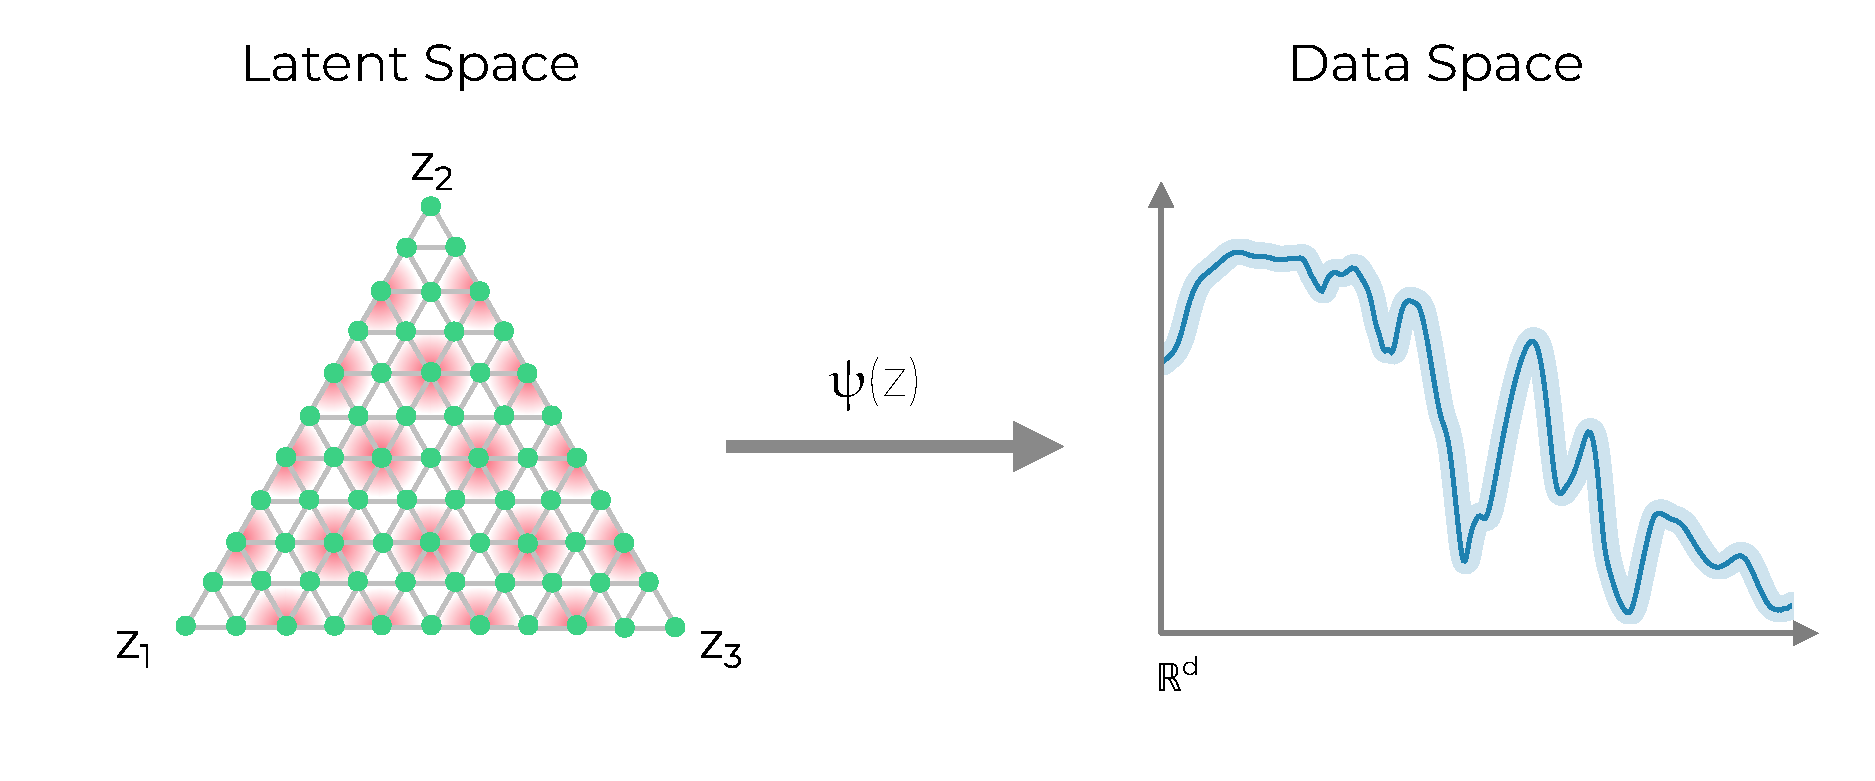
\includegraphics[width=\columnwidth]{methods/gsm/gsm-diagram.pdf}
\caption{Illustration of the GSM. The latent space consists of a grid of $K$-many points (green dots) distributed throughout a simplex with $N_v$ vertices. Barycentric coordinates of each node in the simplex correspond to the relative abundance of $N_v$-many unique sources. Here, $N_v=3$ has been chosen for illustrative purposes. Nodes are mapped into the data space via the map $\psi(z)$ utilizing $M$-many radially symmetric basis functions (red). Spectral variability is estimated via the precision parameter $\beta$ shown here in the data space as a light blue band around the spectrum given by $\psi(z)$.}
\label{fig:gsm-diagram}
\end{figure}  

To further constrain the model, we introduce prior distributions on the weights $\mathbf{W}$. For $m\leq N_v$ we take $W_{dm}\sim\mathcal{N}(0, \lambda_e^{-1})$ corresponding to a zero-mean Gaussian with variance $\lambda_e^{-1}$. For $m>N_v$ we use a zero-mean Laplace distribution, $W_{dm}\sim\dfrac{\lambda_w}{2}\exp(-\lambda_w\lvert W_{dm}\rvert)$, with scale parameter $\lambda_w^{-1}$. Under these choices $\lambda_e$ corresponds to $L_2$ regularization on endmember spectra while $\lambda_w$ corresponds to $L_1$ regularization on the nonlinear activations. In other words, $\lambda_e$ governs the smoothness of the resulting endmembers while $\lambda_w$ encourages sparsity for the nonlinear contributions.

An EM algorithm for the GSM model can now be formulated as follows. Suppose that we have current estimates for the model weights $\mathbf{W}$, mixing coefficients $\pi_k$, and precision parameter $\beta$. During the expectation step we compute the posterior probabilities, that is, the responsibility of each GSM node for each spectrum in the dataset:
\begin{equation}\label{eq:responsibility}
    R_{kn}  = p(z_k \mid x_n, \mathbf{W}, \beta) = \dfrac{\pi_k \, p(x_n \mid z_k, \mathbf{W}, \beta)}{\sum\limits_{k'}^K \pi_{k'} \, p(x_n \mid z_{k'}, \mathbf{W}, \beta)}.
\end{equation}
For the maximization step, we consider the expectation of the penalized complete-data log likelihood given by
\begin{equation}\label{eq:complete-data-llh}
\begin{aligned}
    Q &= \sum_n^N\sum_k^K R_{kn} \left(\ln\pi_k + \frac{D}{2}\ln\left(\frac{\beta}{2\pi}\right) - \frac{\beta}{2}\sum_d^D\left(\sum_m^M W_{dm}\Phi_{km} - X_{nd}\right)^2\right) \\ 
    &\qquad + \frac{N_vD}{2}\ln\left(\frac{\lambda_e}{2\pi}\right) - \frac{\lambda}{2}\sum_d^D \sum_{m=1}^{N_v} W_{dm}^2  \\ 
    &\qquad + (M-N_v)D\ln\left(\dfrac{\lambda_w}{2}\right) - \lambda_w\sum_d^D\sum_{m=N_v+1}^{M} W_{dm}
\end{aligned}
\end{equation}
where $X_{nd}$ is the $d$-th component of the $n$-th spectrum in the dataset. Eq~\ref{eq:complete-data-llh} is then maximized with respect to $\pi_k$, $\beta$, and $\mathbf{W}$ to obtain new parameter values. A detailed overview of the EM procedure can be found in Bishop \cite{bishop-prml}.

For $\pi_k$, optimization can be performed using Lagrange multipliers to maintain the condition that $\sum_k\pi_k=1$. Doing so yields
\begin{equation}\label{eq:pi-update}
    \pi_k^{\text{new}}  = \frac{1}{N}\sum_n R_{kn}
\end{equation}

Optimization of Eq~\ref{eq:complete-data-llh} with respect to $\mathbf{W}$ leads to a linear system which can be solved using standard numerical methods. However, in this form we can not guarantee the non-negativity of $\mathbf{W}$. We therefore take inspiration from the multiplicative updates for NMF introduced by Lee and Seung \cite{nmf-orig}. A gradient-based update for $\mathbf{W}$ would take the form
\begin{equation}
    \mathbf{W}_{\text{new}} = \mathbf{W} + \eta\frac{\partial Q}{\partial \mathbf{W}}
\end{equation}
for some learning rate $\eta$. Differentiating, we obtain
\begin{equation}
    \frac{\partial Q}{\partial \mathbf{W}} = -\beta \mathbf{W}\mathbf{\Phi}^T\mathbf{G}\mathbf{\Phi} - \mathbf{\Lambda} + \beta \mathbf{X}^T\mathbf{R}^T\mathbf{\Phi}
\end{equation}
where $\mathbf{G}$ is a diagonal matrix with $G_{kk} = \sum_n R_{kn}$ and $\mathbf{\Lambda}$ is given by 
\begin{equation}
    \Lambda_{dm} = \begin{cases}
        \lambda_e W_{dm}; & m \leq N_v \\ 
        \lambda_w; & m > N_v
    \end{cases}
\end{equation}
If we allow for individual learning rates $\eta_{dm}$ for each element of $\mathbf{W}$, then choosing 
\begin{equation}
    \eta_{dm} = \frac{W_{dm}}{\left(\beta \mathbf{W}\mathbf{\Phi}^T\mathbf{G}\mathbf{\Phi}\right)_{dm} + \Lambda_{dm}}
\end{equation}
results in update equations for elements of $\mathbf{W}$ given by
\begin{equation}\label{eq:W-update}
    W_{dm}^{new}  = W_{dm} \cdot \dfrac{\left(\beta \mathbf{X}^T\mathbf{R}^T\mathbf{\Phi}\right)_{dm}}{\left(\beta \mathbf{W}\mathbf{\Phi}^T\mathbf{G}\mathbf{\Phi}\right)_{dm} + \Lambda_{dm}}
\end{equation}
From Eq~\ref{eq:W-update}, it is clear that we are multiplying $W_{dm}$ by non-negative values and therefore, $W_{dm}$ remains non-negative.

Finally, optimizing Eq~\ref{eq:complete-data-llh} with respect to $\beta$ yields
\begin{equation}\label{eq:beta-update}
    \frac{1}{\beta^{\text{new}}}  = \frac{1}{ND}\sum\limits_n^N\sum\limits_k^K R_{kn}\lVert \psi(z_k; \mathbf{W}) - x_n \rVert^2.
\end{equation}
The expectation and maximization steps are repeated in turn until $Q$ converges to a predetermined tolerance level.

\subsection{Implementation Details}

The mixing coefficients are initially chosen so that $\pi_k = \frac{1}{K}$.

- Linear Method

- Nonlinear Method

- Mixed Method


\section{Experiments}\label{sec:experiments}
\subsection{Linear Mixing: Comparison to NMF}
- describe USGS data
- describe NMF method (for comparisson)
- describe evaluation criteria


\begin{figure}[H]
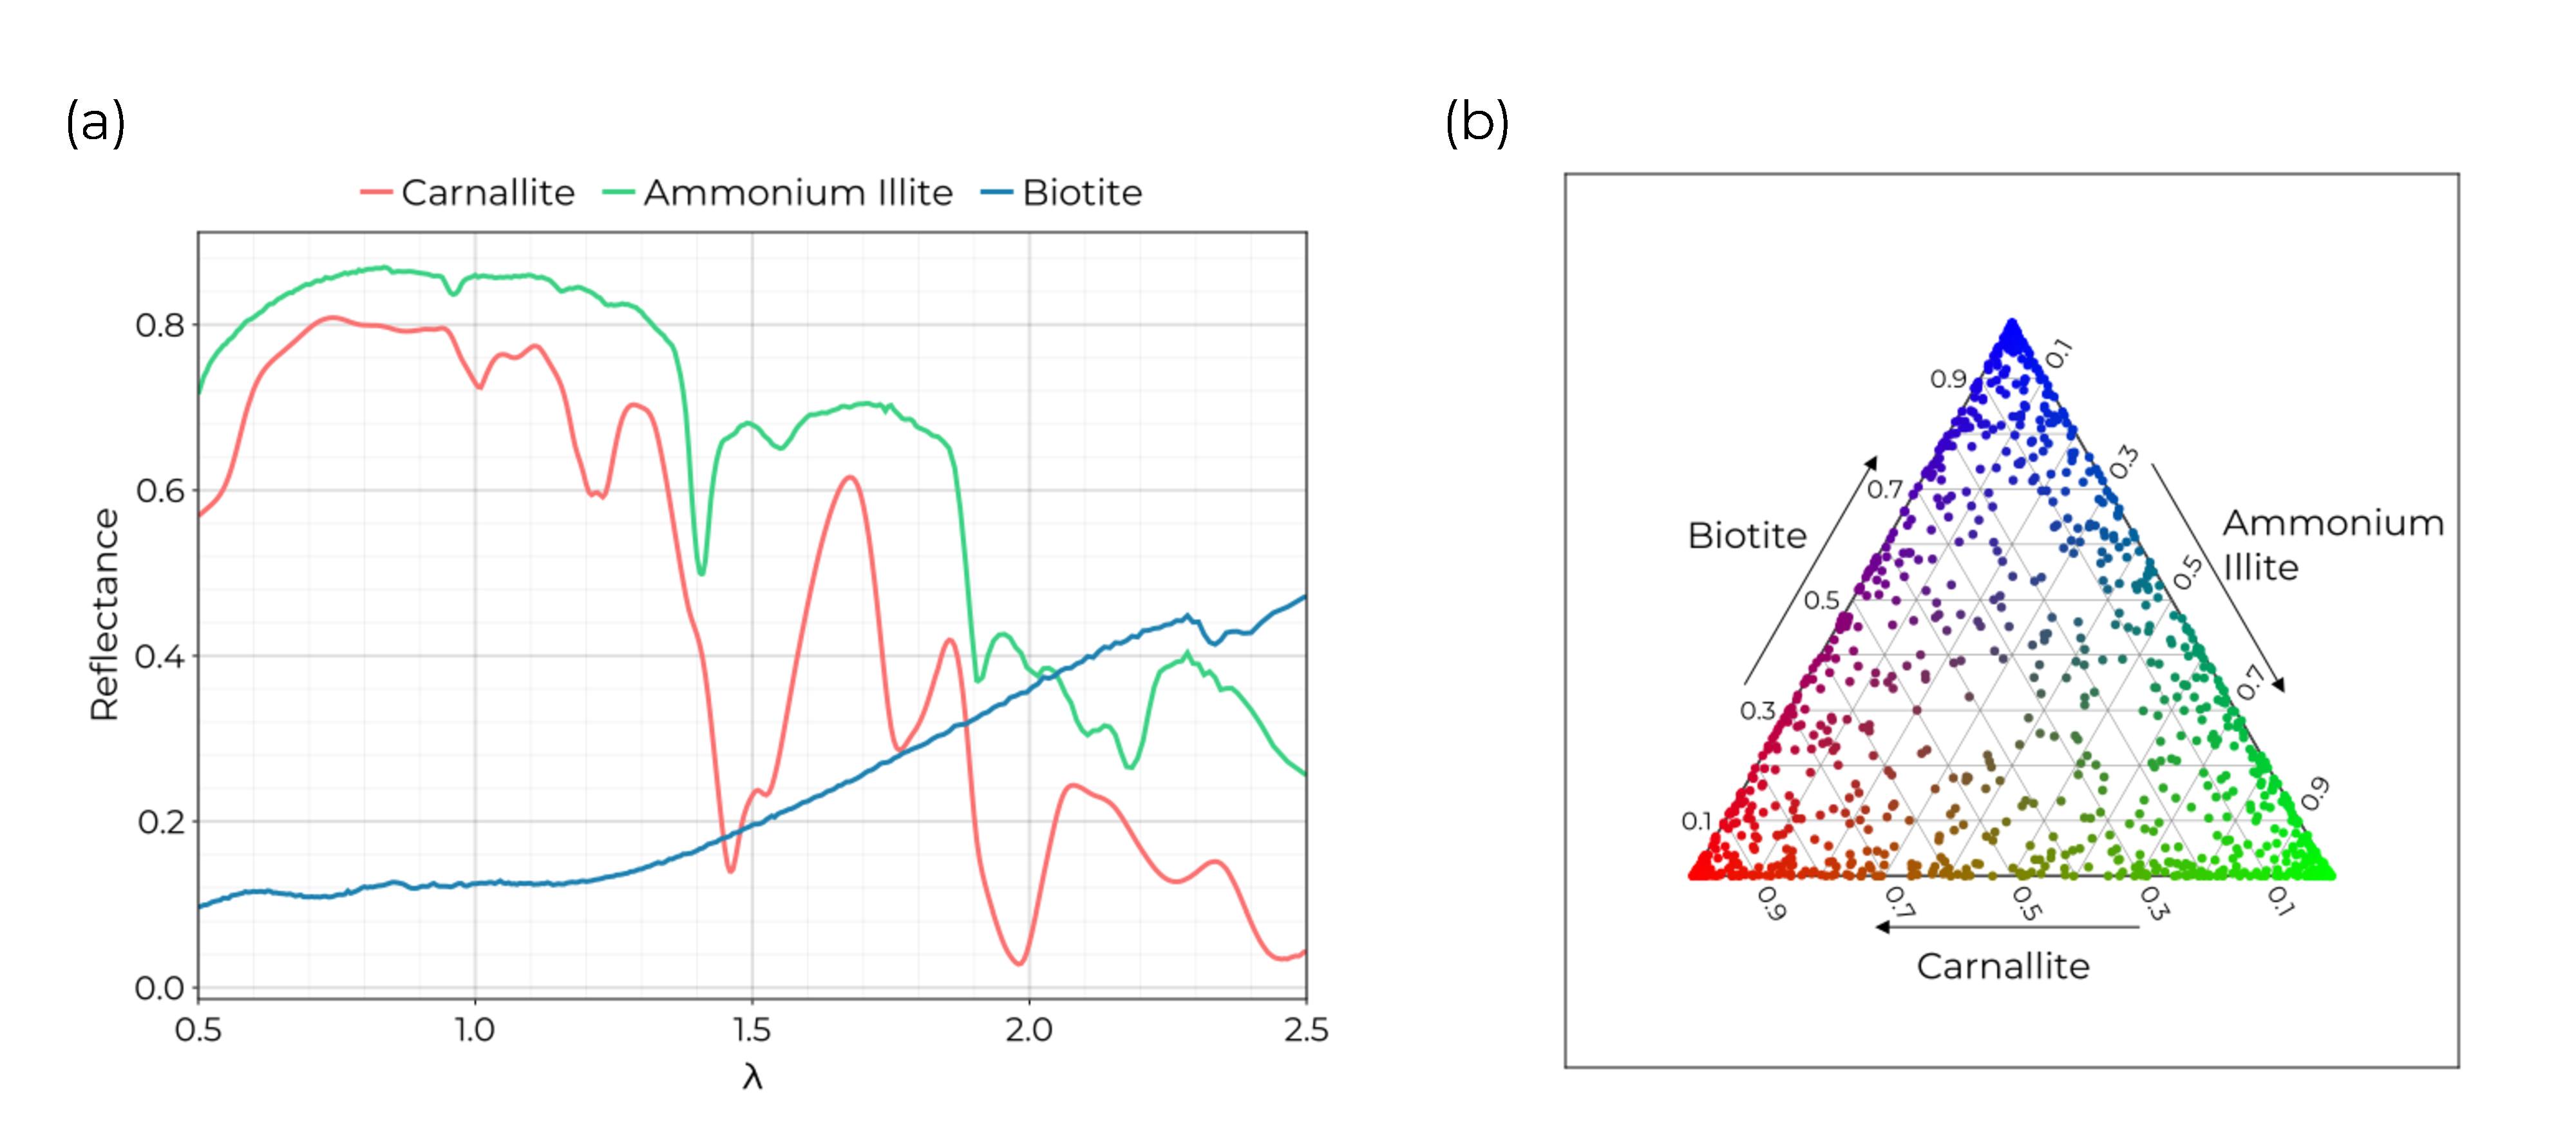
\includegraphics[width=\columnwidth]{methods/usgs/usgs-dataset.pdf}
\caption{Synthetic dataset from USGS spectra. \label{fig:usgs-data}}
\end{figure}  




\subsection{Nonlinear Mixing: Water Contaminant Identification}
- describe robot team data collection and processing
- describe 



\begin{figure}[H]
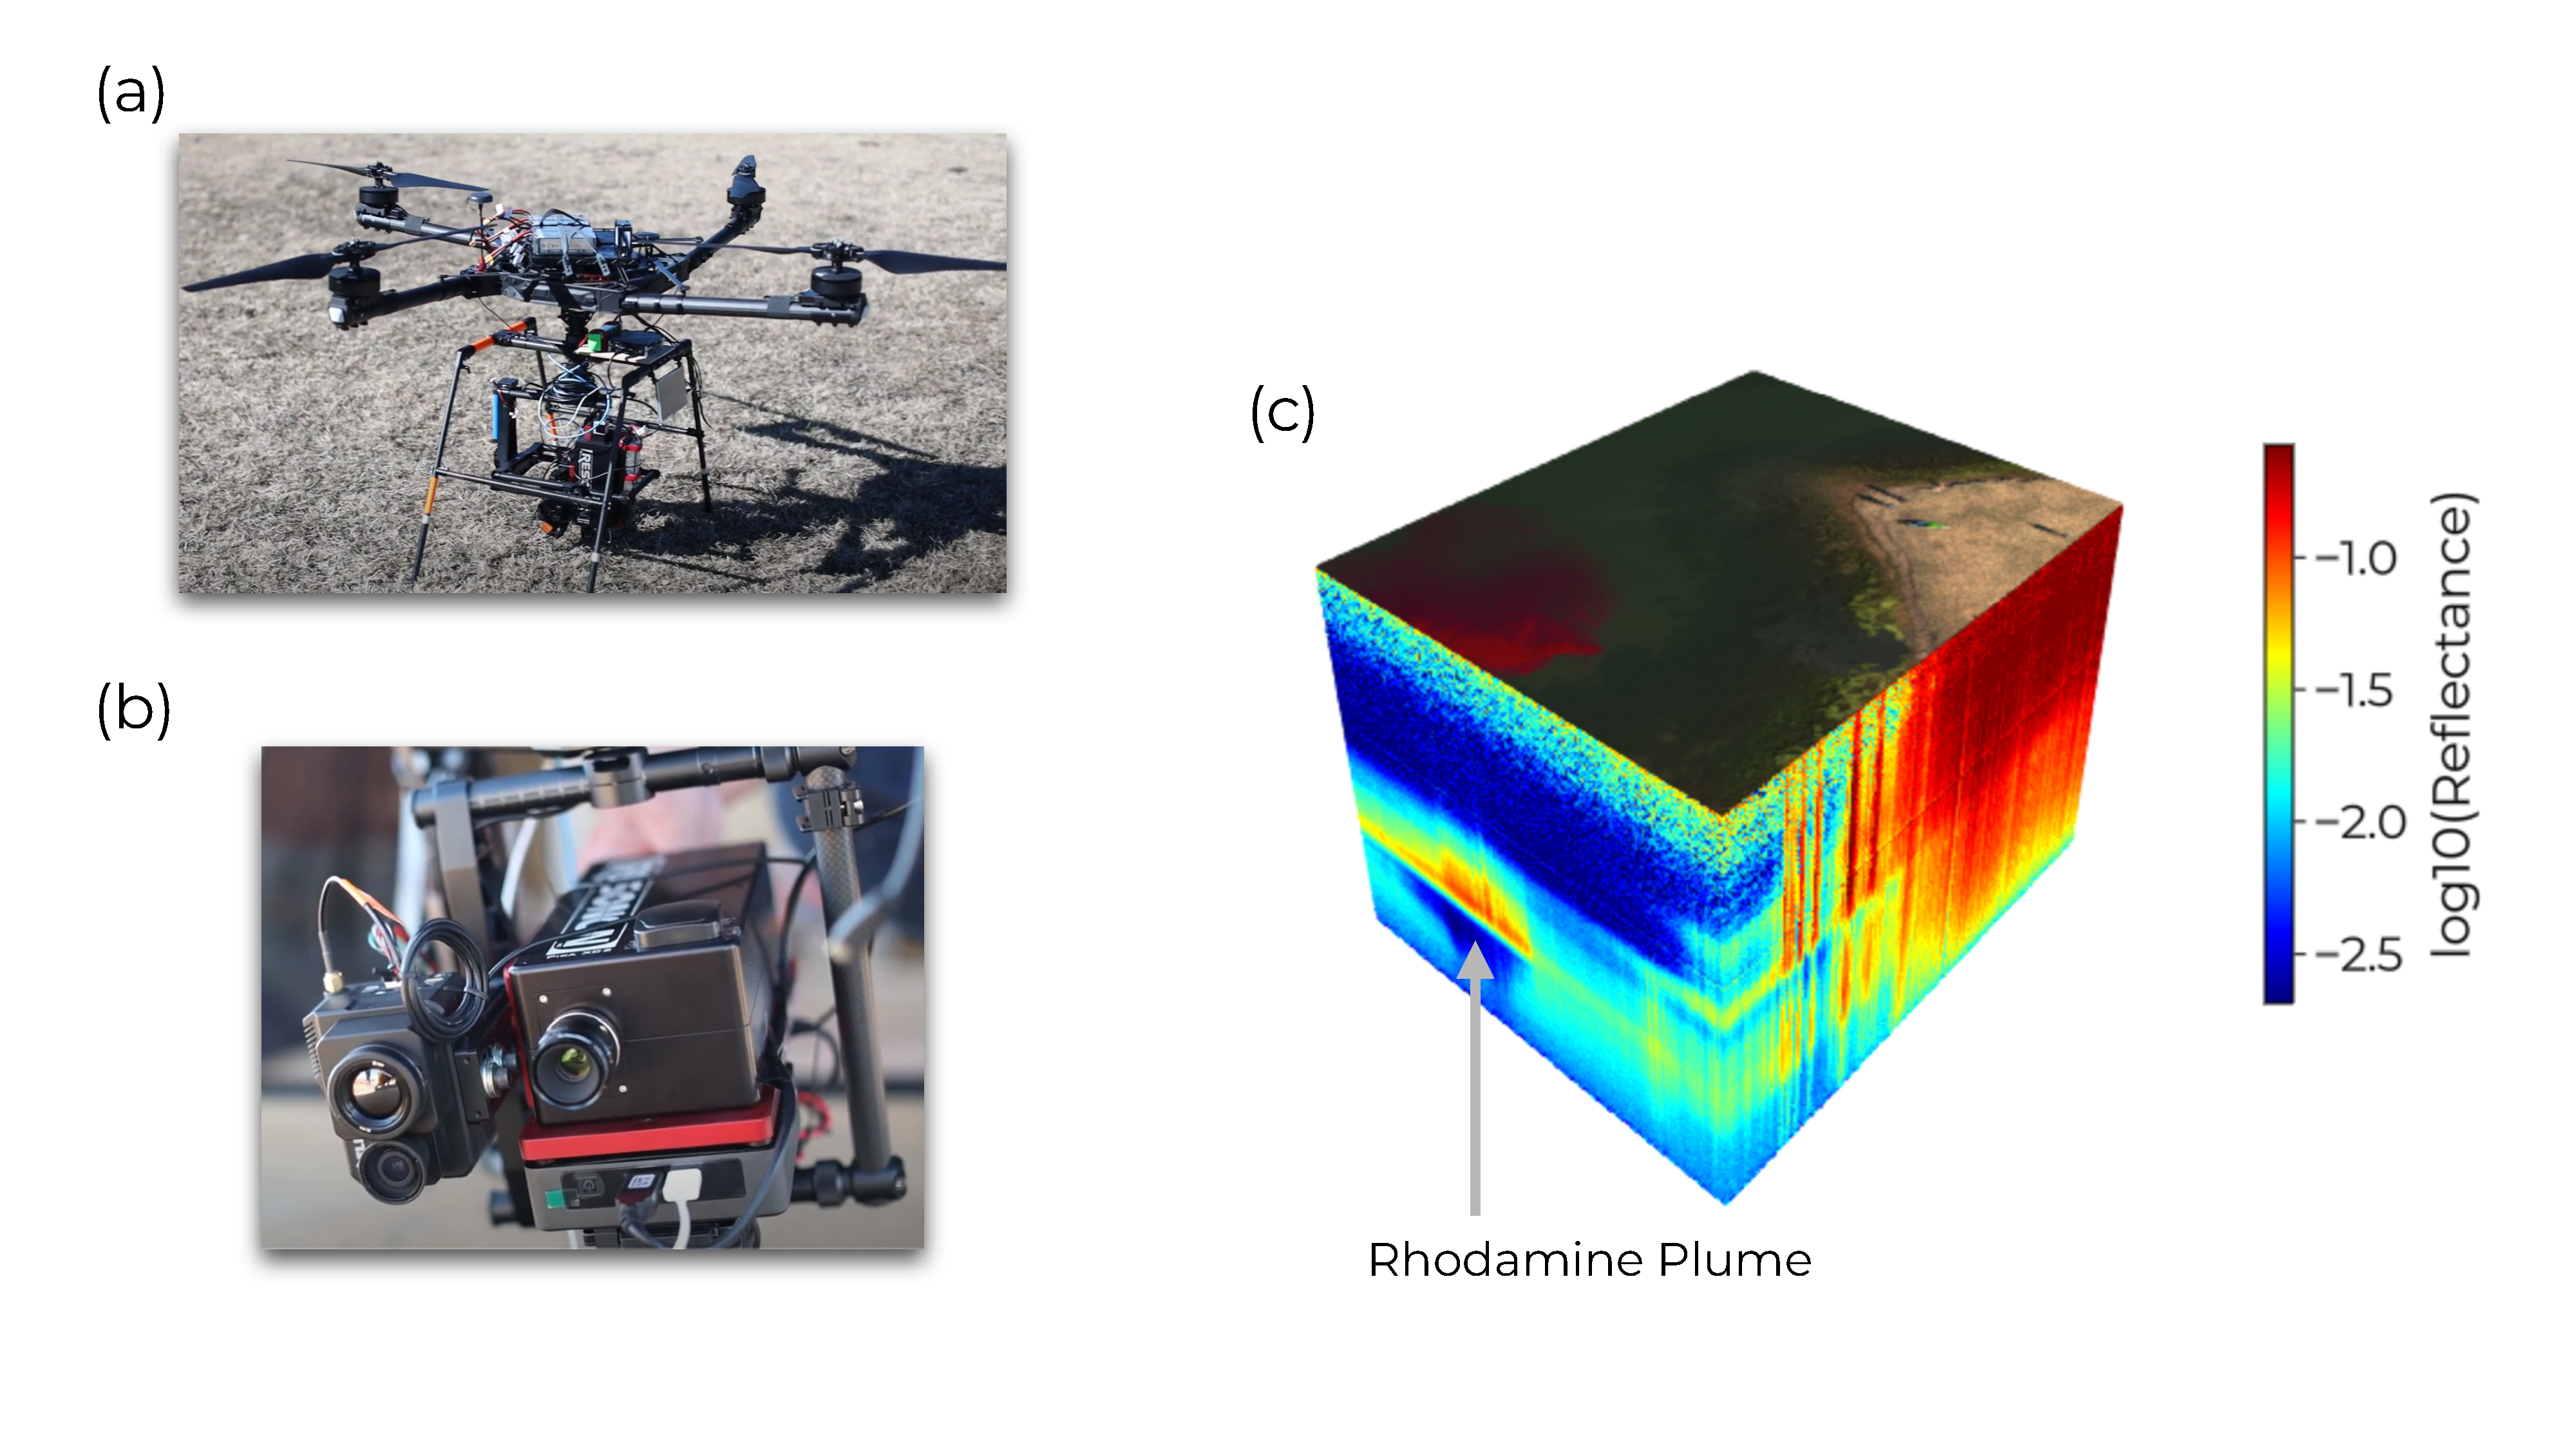
\includegraphics[width=\columnwidth]{methods/robot-team/robot-team-overview.pdf}
\caption{Robot team dataset. \label{fig:robotteam-data}}
\end{figure}  



\section{Results}\label{sec:results}
\subsection{Linear Mixing}

\begin{figure}[H]
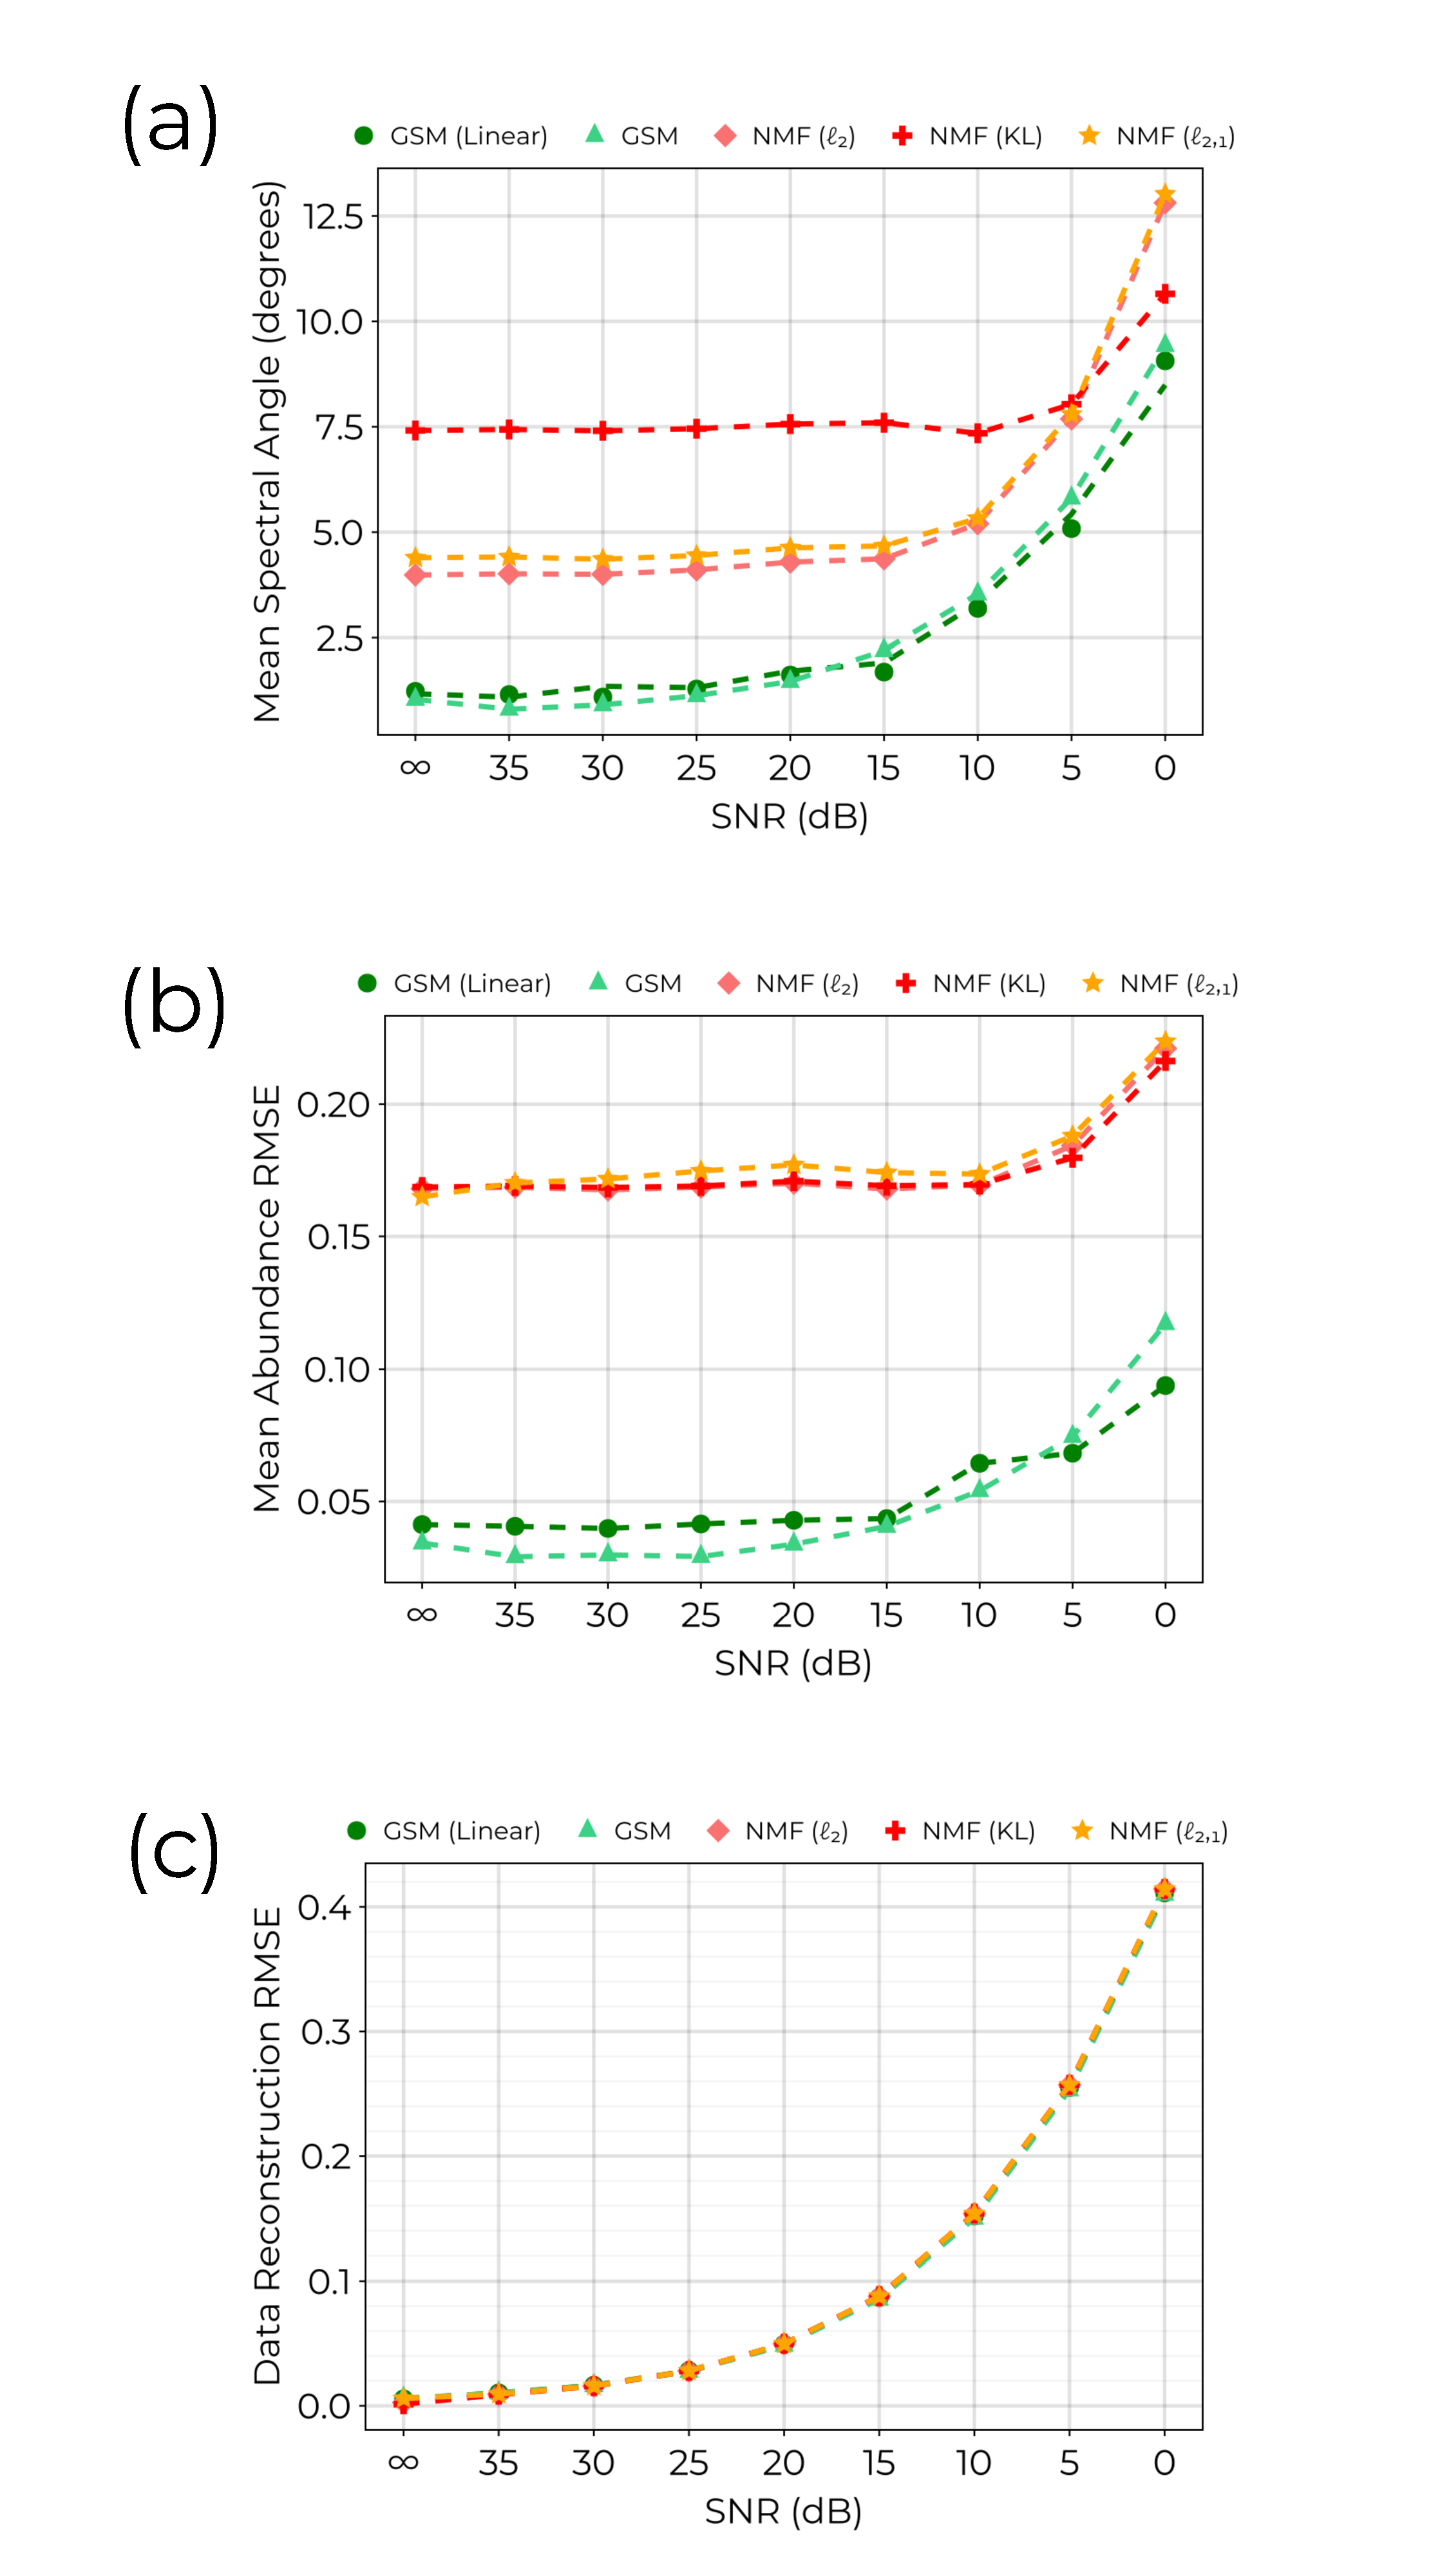
\includegraphics[width=\columnwidth]{results/usgs/fit-comparison.pdf}
\caption{Comparison of GSM against NMF on simulated USGS dataset. \label{fig:usgs-fits}}
\end{figure}  


\begin{figure}[H]
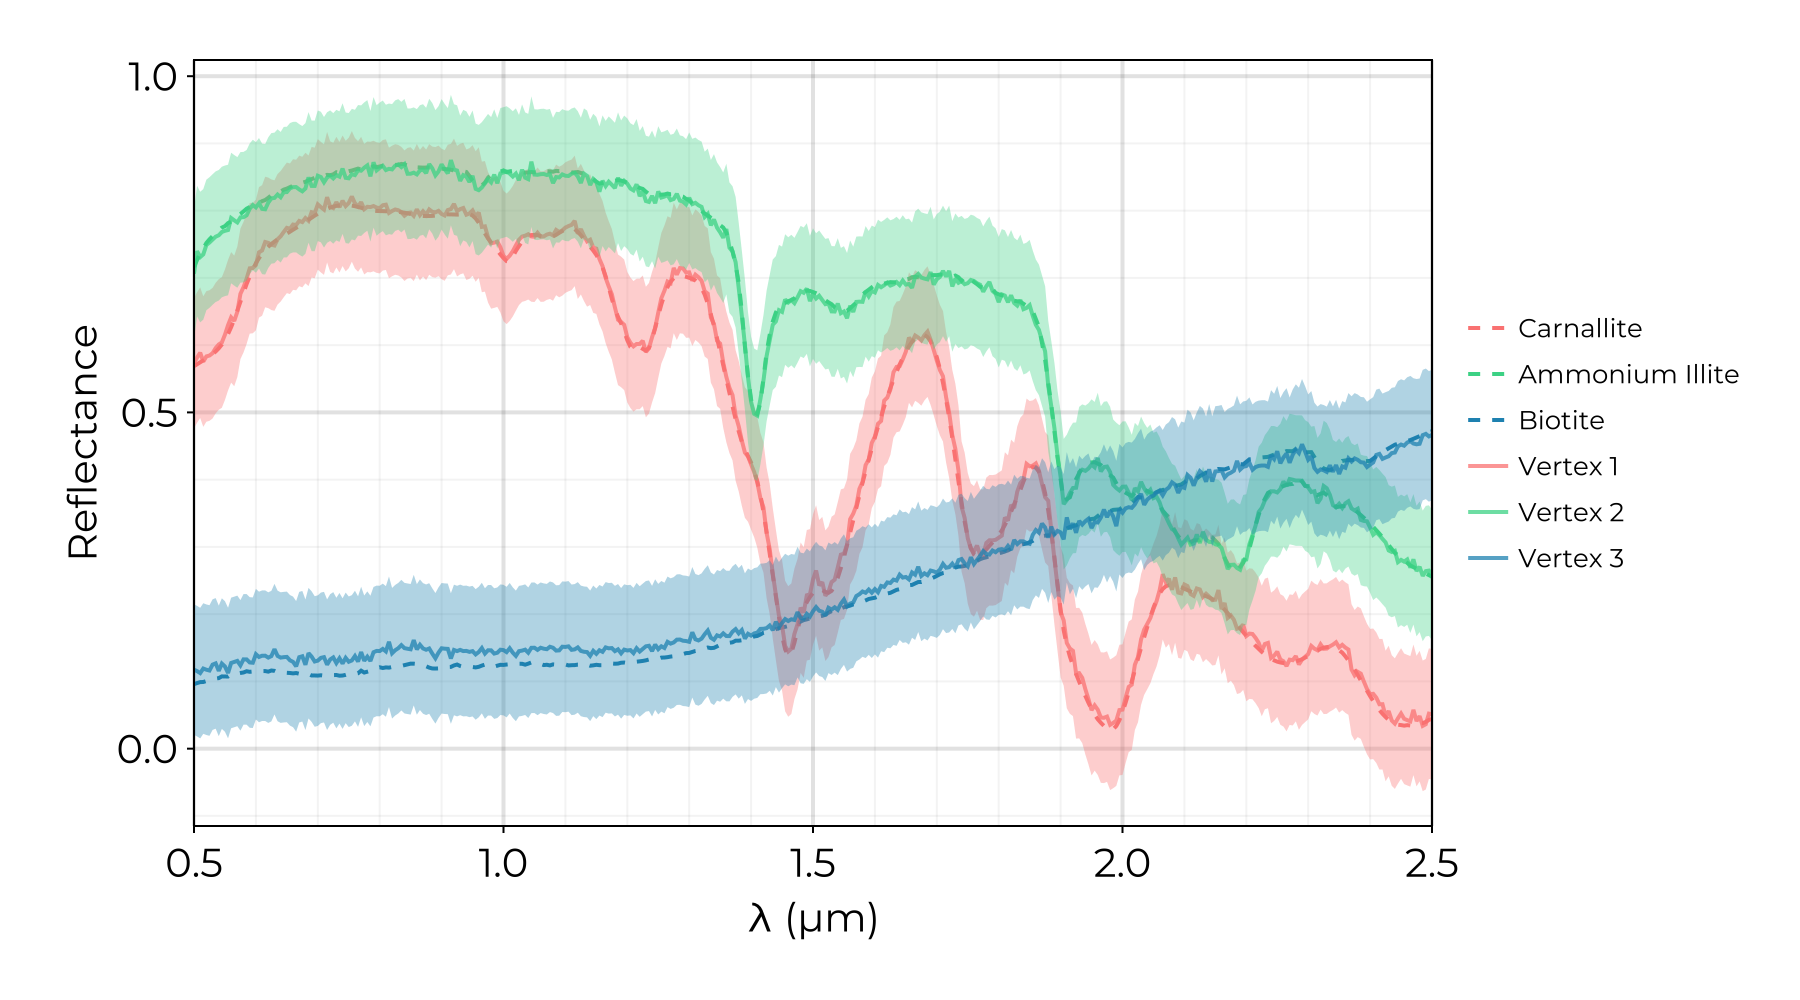
\includegraphics[width=\columnwidth]{results/usgs/extracted-endmembers.png}
\caption{Endmembers extracted using GSM for simulated USGS dataset with SNR$=20$. \label{fig:usgs-endmembers}}
\end{figure}  


\subsection{Nonlinear Mixing: Rhodamine Dye Plume}

Exploratory data analysis: 
\begin{figure}[H]
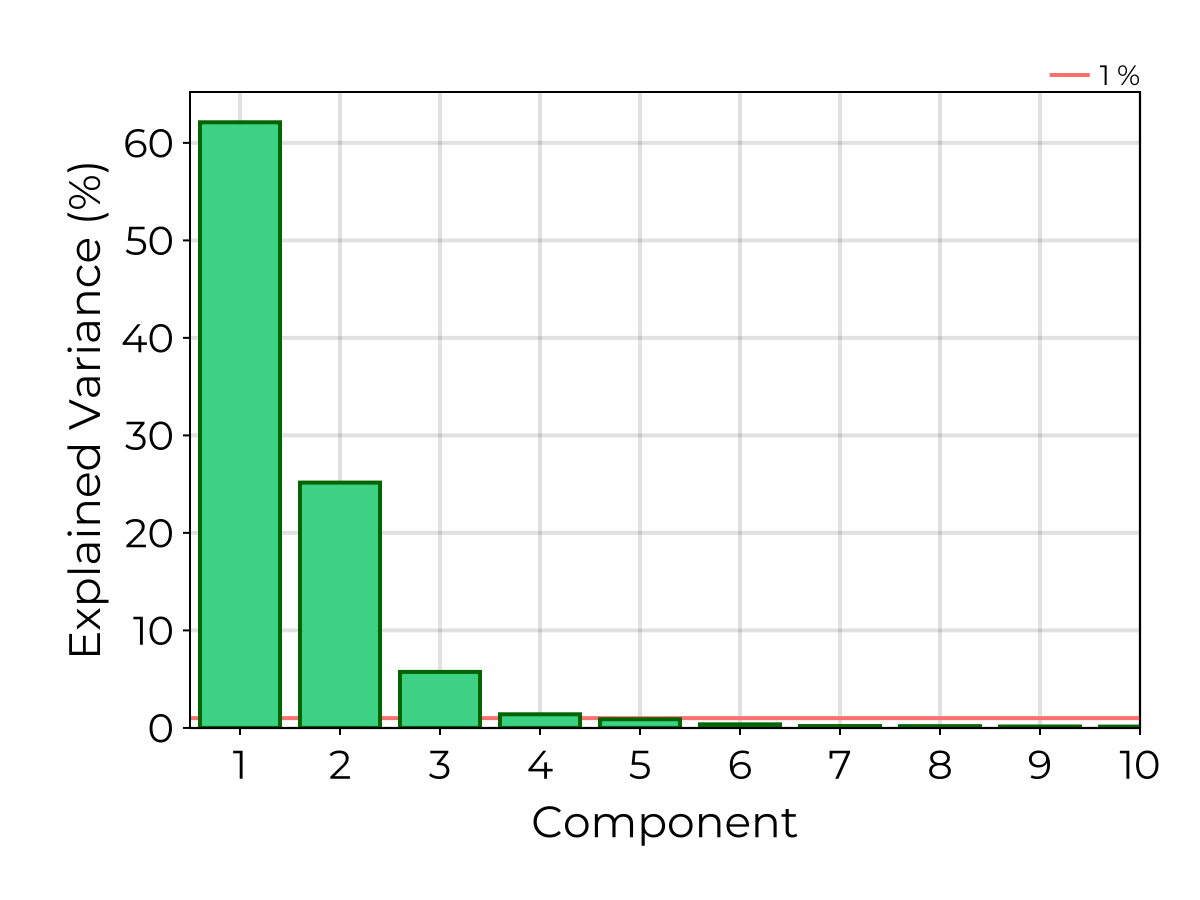
\includegraphics[width=0.60\columnwidth]{results/robot-team/pca-variance.png}
\caption{Explained variance of PCA components for robot team dataset. A red horizontal line is superimposed on the plot indicating an explained variance of $1\%$. \label{fig:robot-team-pca}}
\end{figure}  

\begin{table}[H] 
\caption{Hyperparameter optimization: Multiple models were trained to identify optimal hyperparameter values for the GSM applied to the water spectra dataset. Here we report the top $10$ models ranked according the the BIC.}
\label{table:fit-comparison}
\begin{tabularx}{\textwidth}{CCCCCC}
\toprule
\textbf{$N_v$}	& \textbf{$\lambda_e$}	& \textbf{$\lambda_w$} & \textbf{BIC} & \textbf{AIC} & \textbf{Reconstruction RMSE}\\
\midrule
$3$ & $0.01$    & $1.0$     & $-6.195\times10^7$   & $-6.269\times10^7$   & $0.000989$ \\
$3$	& $0.001$   & $1.0$     & $-6.194\times10^7$   & $-6.268\times10^7$   & $0.000989$ \\
$3$	& $0.1$     & $1.0$	    & $-6.192\times10^7$   & $-6.265\times10^7$   & $0.000991$ \\
$3$	& $1.0$     & $1.0$	    & $-6.186\times10^7$   & $-6.260\times10^7$   & $0.001190$ \\
$4$	& $1.0$     & $1.0$	    & $-6.181\times10^7$   & $-6.255\times10^7$   & $0.001002$ \\
$4$	& $0.1$     & $1.0$	    & $-6.175\times10^7$   & $-6.249\times10^7$   & $0.001008$ \\
$4$	& $0.01$    & $1.0$     & $-6.173\times10^7$   & $-6.247\times10^7$   & $0.001009$ \\ 
$4$	& $0.001$   & $1.0$     & $-6.173\times10^7$   & $-6.247\times10^7$   & $0.001009$ \\
$4$	& $0.1$     & $10.0$    & $-6.171\times10^7$   & $-6.245\times10^7$   & $0.001011$ \\
$3$	& $1.0$     & $10.0$    & $-6.166\times10^7$   & $-6.239\times10^7$   & $0.001014$ \\
\bottomrule
\end{tabularx}
\end{table}


\begin{figure}[H]
\begin{adjustwidth}{-\extralength}{0cm}
\centering
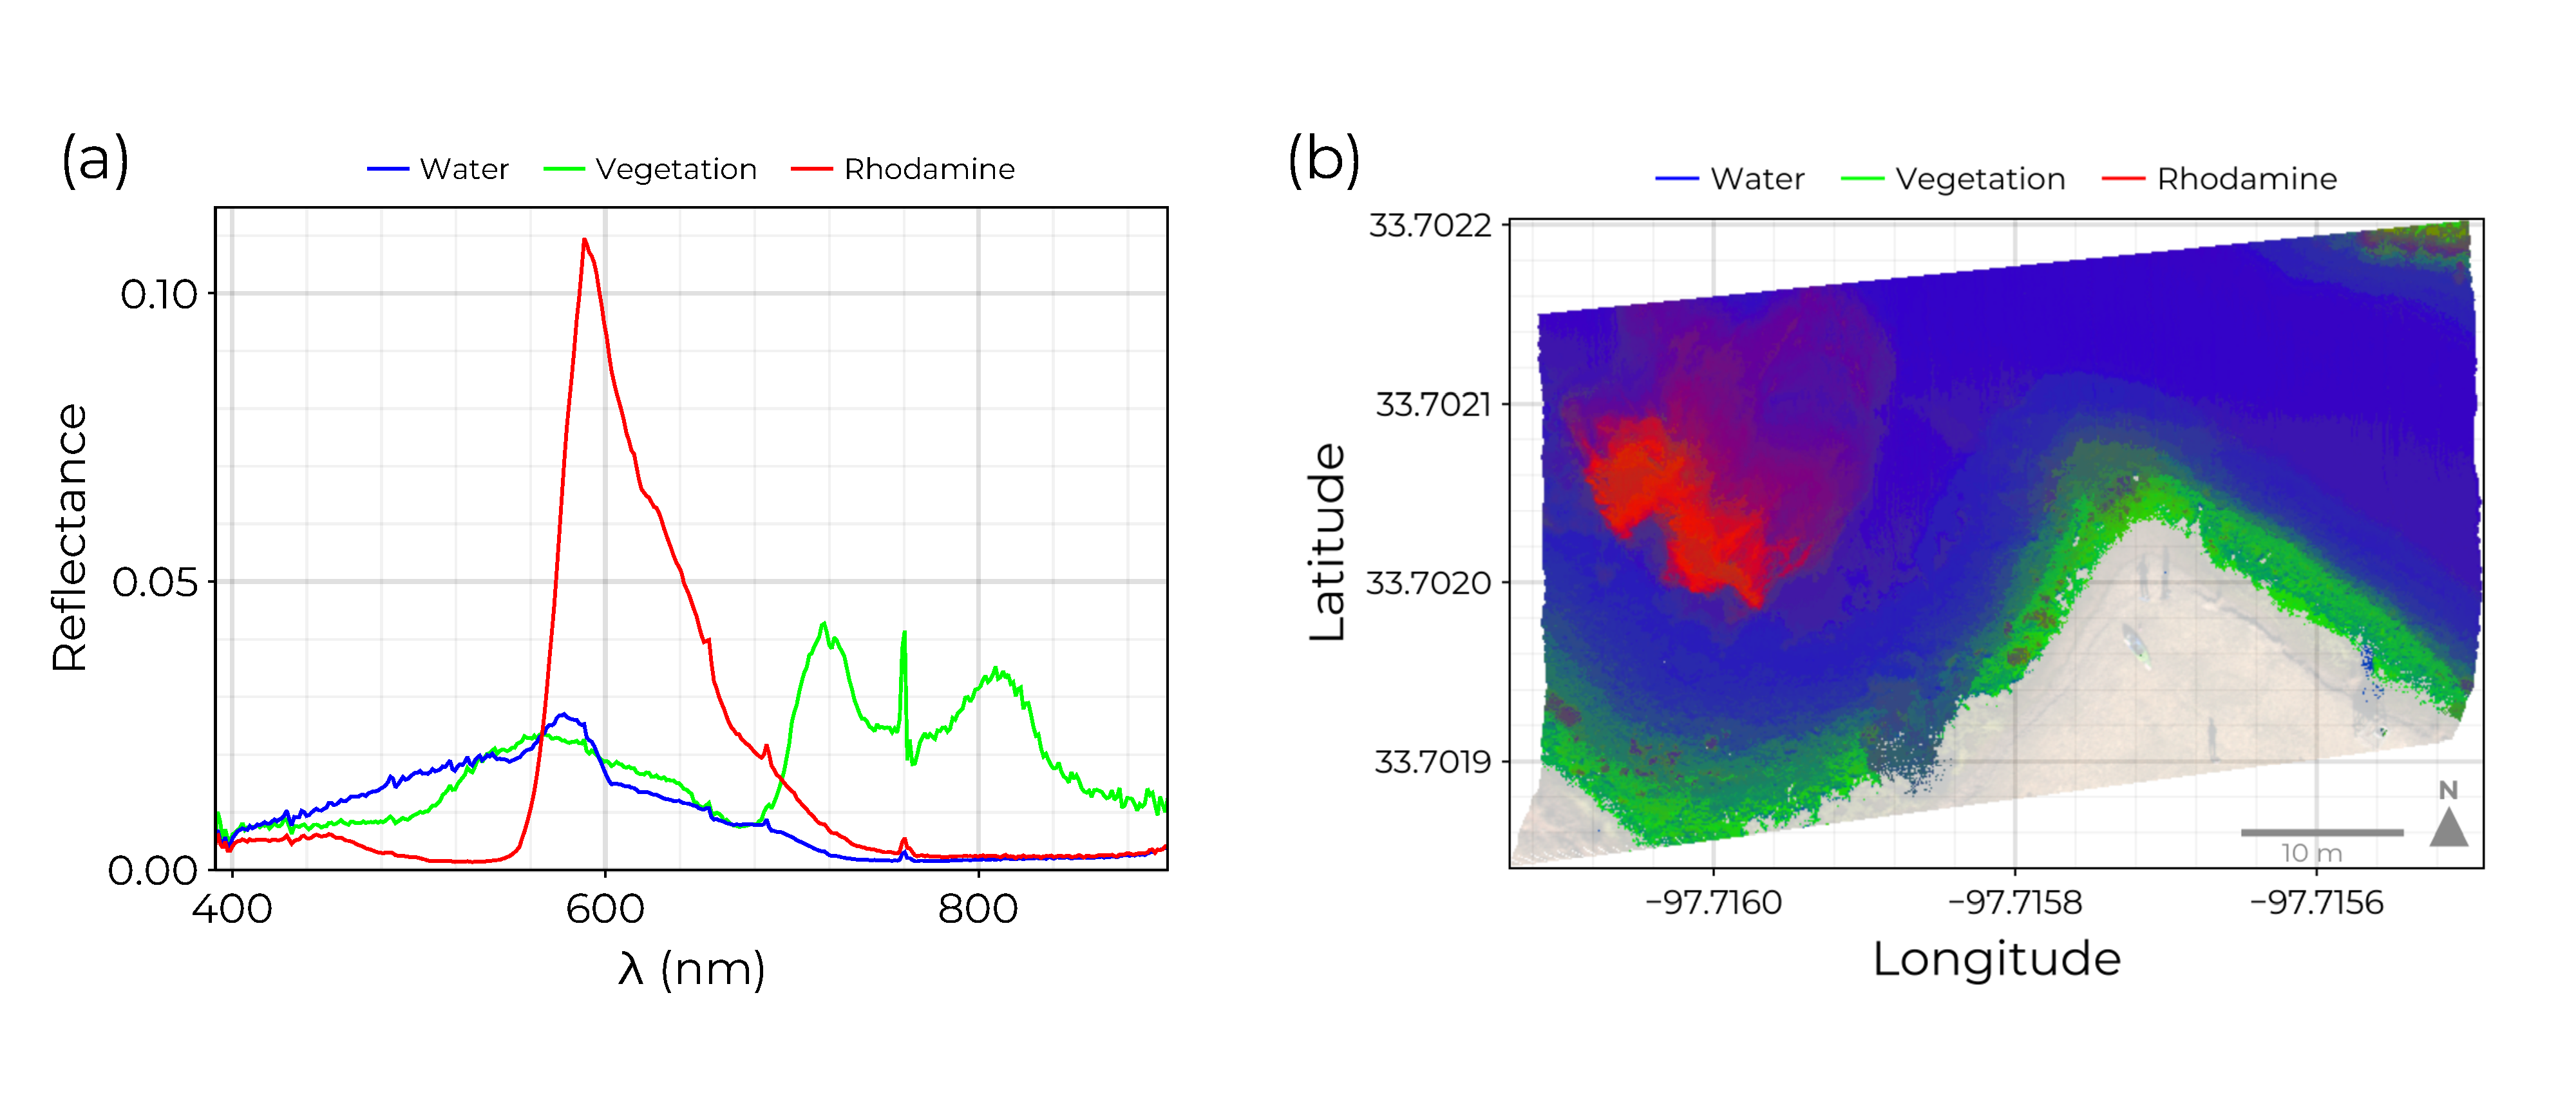
\includegraphics[width=1.25\columnwidth]{results/robot-team/extracted-endmembers.pdf}
\end{adjustwidth}
\caption{Nonlinear GSM applied to water spectra: \textbf{(a)} Spectra corresponding to maximum abundances for each vertex in the trained GSM identified for as water, near-shore vegetation, and rhodamine dye sources. \textbf{(b)} The original hyperspectral datacube segmented according to the relative abundance of each endmember. Each water pixel defined by an NDWI $\geq 0.25$ is colored by smoothing interpolating between red, green, and blue colors corresponding to the relative abundance estimated for rhodamine, vegetation, and water spectra.}
\label{fig:robot-team-endmembers}
\end{figure}  

\newpage
\begin{figure}[H]
\begin{adjustwidth}{-\extralength}{0cm}
\centering
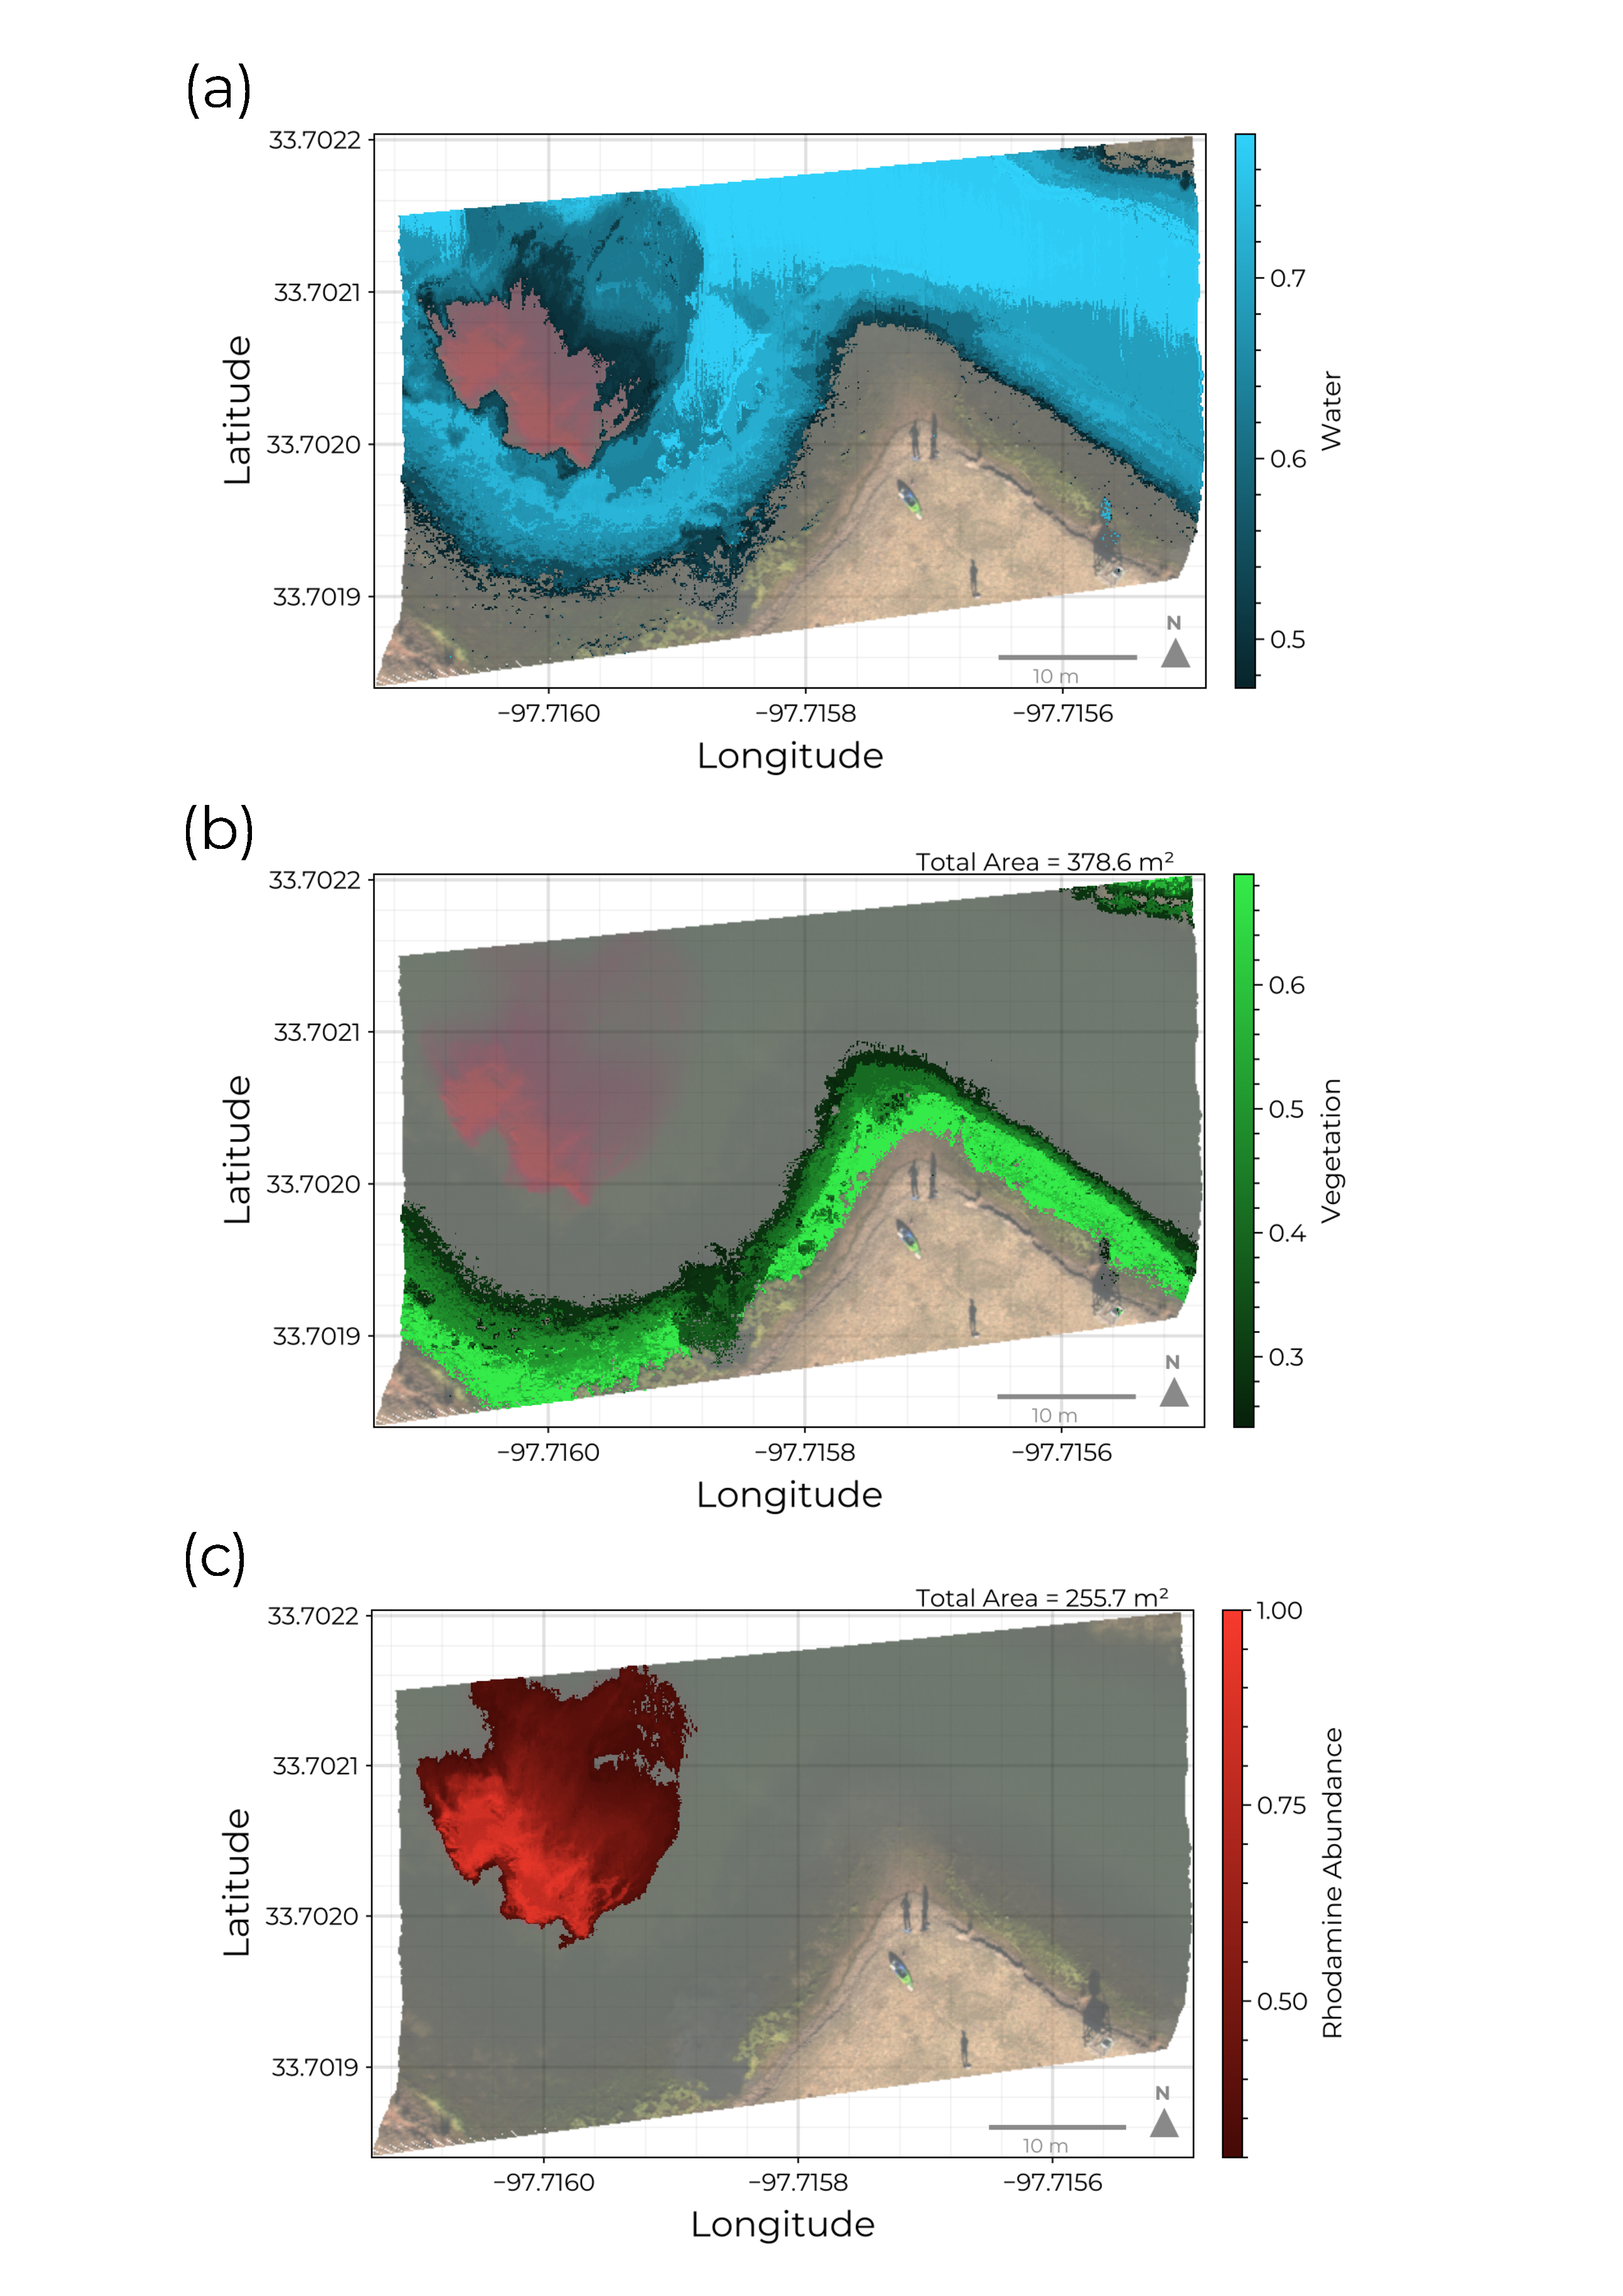
\includegraphics[width=\columnwidth]{results/robot-team/endmember-abundances.pdf}
\caption{Endmember distributions: \textbf{(a)} The distribution of abundance for the water class. This source dominates in the center of the water and decreases towards the edge of the pond where surface vegetation begins to dominate the reflectance signal. We note that the water abundance decreases near  the edge of the rhodamine plume reflecting dye mixing and diffusion. \textbf{(b)} The distribution of vegetation. This signal includes filamentous blue-green algae observed to accumulate in shallow waters near the shore. \textbf{(c)} The rhodamine dye plume extent segmented from the HSI. The total area for near-shore vegetation and rhodamine are estimated to be $378.6$ $\text{m}^2$ and $255.7$ $\text{m}^2$ respectively.}
\end{adjustwidth}
\label{fig:endmember-abundance-dist}
\end{figure}  
\newpage


\begin{figure}[H]
\begin{adjustwidth}{-\extralength}{0cm}
\centering
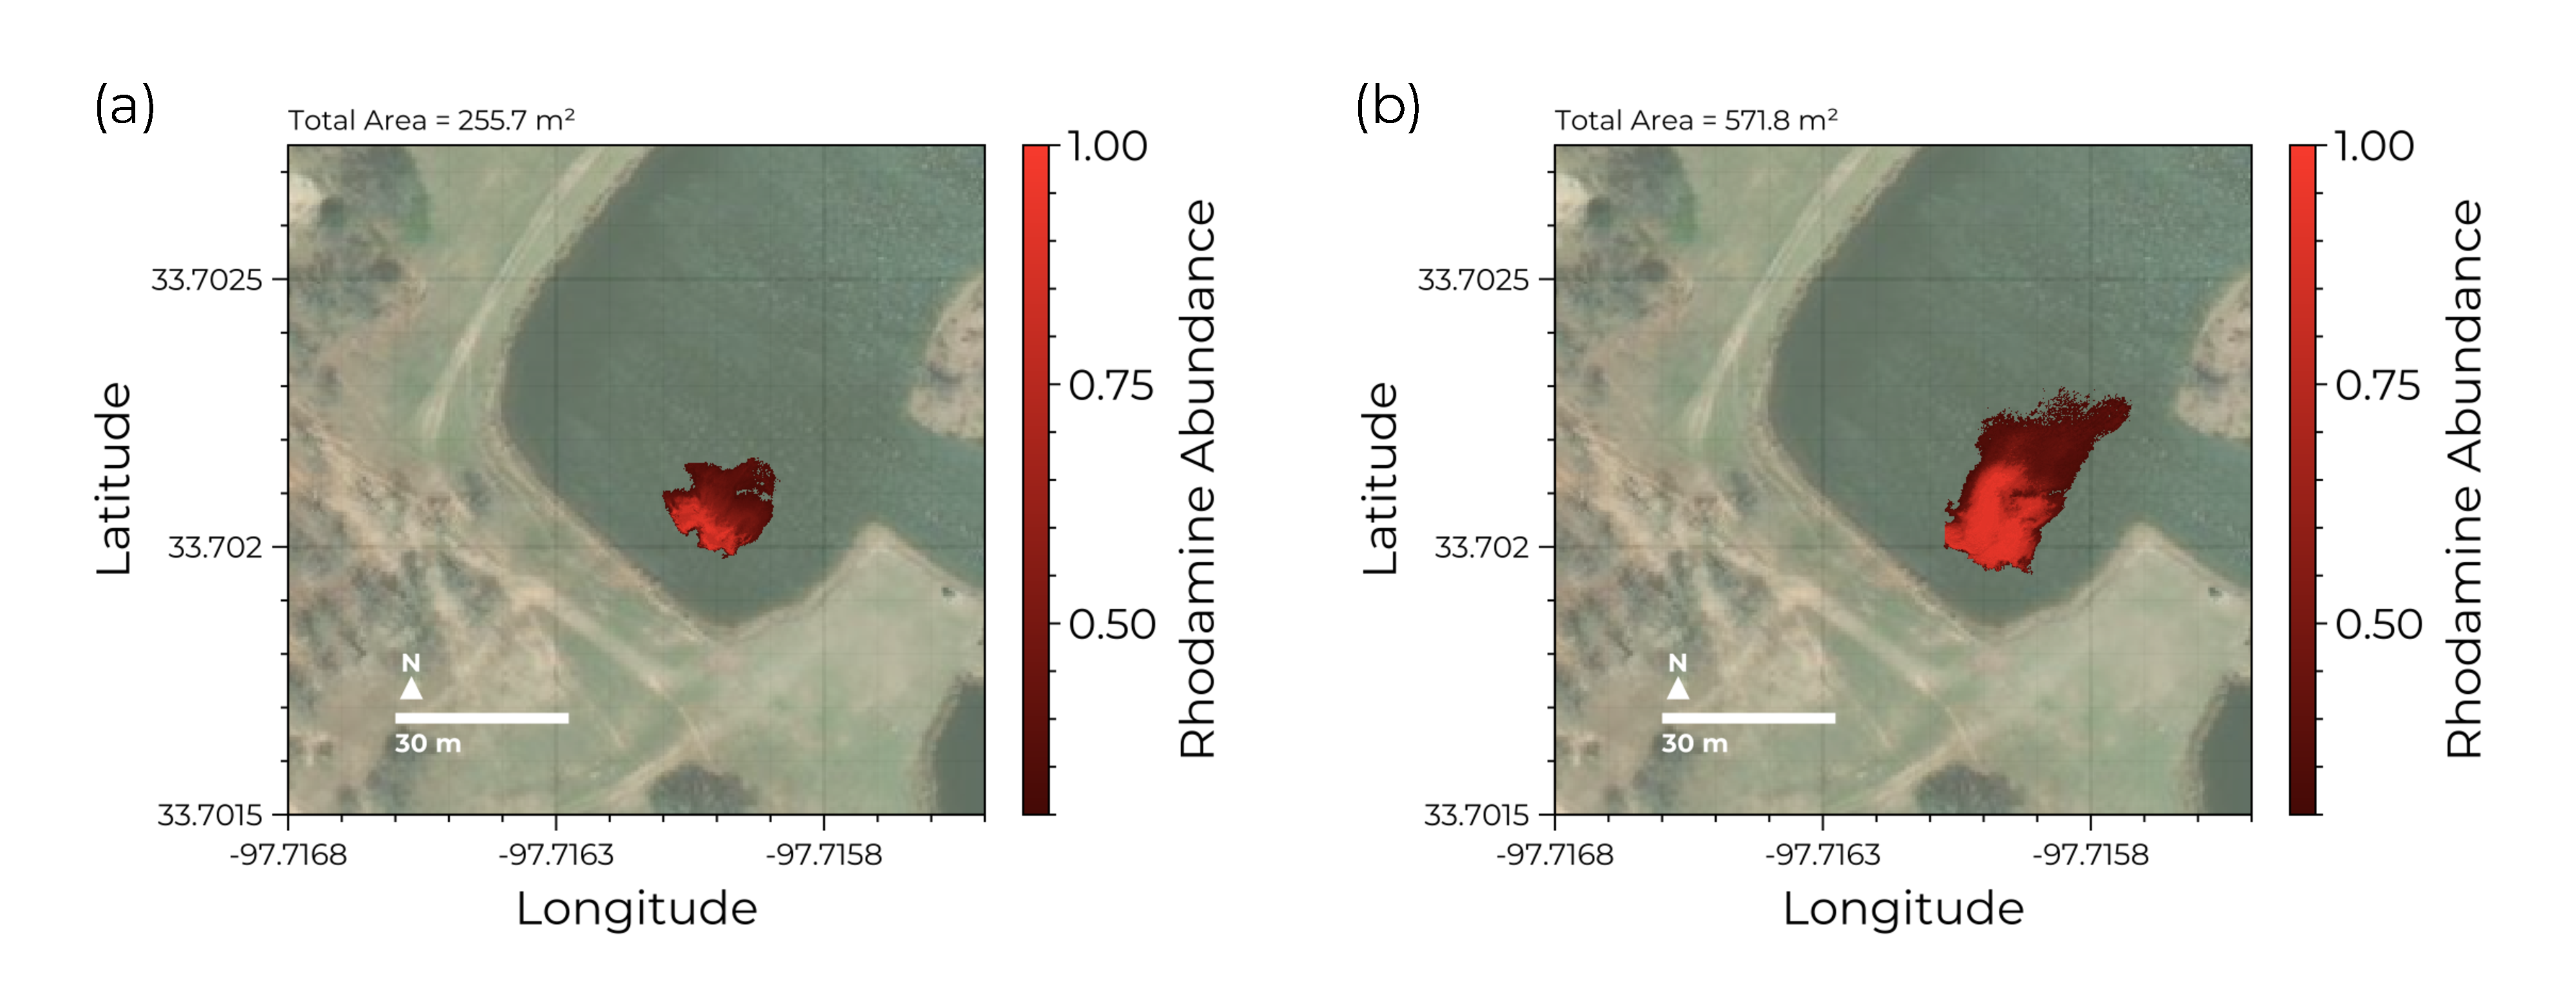
\includegraphics[width=1.25\columnwidth]{results/robot-team/plume-evo.pdf}
\end{adjustwidth}
\caption{Rhodamine plume evolution: Using the trained GSM we can track the dispersion of the rhodamine dye plume between successive drone flights. \textbf{(a)} The initial plume distribution after release. Here the dye subsumes an area of $255.7$ $\text{m}^2$. \textbf{(b)} The same plume imaged 15 minutes later now extends across an area of $571.8$ $\text{m}^2$}
\label{fig:plume-evo}
\end{figure}  


\section{Discussion}\label{sec:disucssion}

- Comparison to NMF on linear mixing problem
    - note that there are many versions of NMF with different constraints/regularization. The purpose here was to show that GSM is at least \textit{comparable} to NMF for linear unmixing problems
    - Further note that both NMF and GSM do not rely on assumption of pure pixels (unlike VCA and other methods) 
    - GSM also allows estimation of endmember variability via the precision parameter $\beta$ i.e. nodes in data-space follow Gaussian distribution with $\sigma = \sqrt{\beta^{-1}}$

- Nonlinear GSM for robot team 
    - discuss identification of rhodamine plume and easy abundance mapping via the embedding coordinate
    - discuss intrinsic dimensionality identification via abundance sparsity and BIC
    - Discuss identification of non-linearity \textit{strength} via regularization parameter and BIC.
    - reconstruction rmse can also be used to evaluate the relative performance for fixed model size (i.e. k and m) with varying regularization strength

- Limitations of the GSM
    - slow training due to computation of dinstance matrix between full dataset and embedding space
    - An incremental version of the EM procedure as described in \cite{gtm-developments} can speed this up by considering batches $X_b$ of $X$ and performing only a partial E-step by updating responsibilities corresponding to the data batch
    - However, M step still involves the "full" responsibility matrix. 
    - This can be addressed by taking an ensembling approach as described in \cite{parallel-gtm} where multiple GTM are trained on subsets of $X$ and the results are averaged. 
    - More generally, we may consider a mixture-of-GTMs as briefly desribed in \cite{gtm-orig} whereby the overall density is given as 
    \begin{equation}
        p(\mathbf{x}) = \sum_r P(r)p(\mathbf{x}\vert r)
    \end{equation}
    where there are $r$ individual GTM models with mixing coefficients $P(r)$ such that $\sum_r P(r) =1$

- Other potential extensions to GSM model
     - Adapt latent space  to allow for points whose barycentric coordinates sum to less than 1 in order to account for lighting effects (shouldn't matter for reflectance but would matter for radiance depending on incident light). This is the $\gamma$ factor that shows up in some of the mixing papers.

- Discuss other applications of the GSM
    - Optimal route planning for in-situ data collection based on prize-collecting travelling salesman problem, i.e. construct a route which maximizies area traversed in GSM latent space (e.g. the n-simplex). 
    - Applications to source apportionment, e.g. linear GSM can be used for standard source apportionment problems (no reactions) and nonlinear GSM may be useful for modeling scenarios with additional complications due to reactions and during transport from source to receptor.

\section{Conclusions}\label{sec:conclusions}


\section{Patents}

\textcolor{red}{UPDATE ME!}

%%%%%%%%%%%%%%%%%%%%%%%%%%%%%%%%%%%%%%%%%%
\vspace{6pt} 


%%%%%%%%%%%%%%%%%%%%%%%%%%%%%%%%%%%%%%%%%%
\authorcontributions{Methodology, J.W.; conceptualization, J.W.; software, J.W.; validation, J.W.; formal analysis, J.W.; investigation J.W.; resources, D.J.L.; writing---original draft preparation, J.W.; writing---review and editing, J.W. and D.J.L.; visualization, J.W.; supervision, D.J.L.; project administration, D.J.L.; funding acquisition, D.J.L. All authors have read and agreed to the published version of the manuscript.
}


\funding{\textcolor{red}{Please add: ``This research received no external funding'' or ``This research was funded by NAME OF FUNDER grant number XXX.'' and  and ``The APC was funded by XXX''. Check carefully that the details given are accurate and use the standard spelling of funding agency names at \url{https://search.crossref.org/funding}, any errors may affect your future funding.}}


\institutionalreview{Not applicable.}

\informedconsent{Not applicable.}


\dataavailability{\textcolor{red}{We encourage all authors of articles published in MDPI journals to share their research data. In this section, please provide details regarding where data supporting reported results can be found, including links to publicly archived datasets analyzed or generated during the study. Where no new data were created, or where data is unavailable due to privacy or ethical restrictions, a statement is still required. Suggested Data Availability Statements are available in section ``MDPI Research Data Policies'' at \url{https://www.mdpi.com/ethics}.}}


\acknowledgments{\textcolor{red}{In this section you can acknowledge any support given which is not covered by the author contribution or funding sections. This may include administrative and technical support, or donations in kind (e.g., materials used for experiments).}}

\conflictsofinterest{The authors declare no conflicts of interest.}
 

%%%%%%%%%%%%%%%%%%%%%%%%%%%%%%%%%%%%%%%%%%
%% Optional

%% Only for journal Encyclopedia
%\entrylink{The Link to this entry published on the encyclopedia platform.}

\abbreviations{Abbreviations}{
The following abbreviations are used in this manuscript:\\

\noindent
\begin{tabular}{@{}ll}
PRISMA & Hyperspectral Precuror of the Application Mission \\
EnMAP & Environmental Mapping and Analysis Program \\
PACE & Plankton, Aerosol, Cloud, ocean Ecosystem \\
CHIME & Copernicus Hyperspectral Imaging Mission for the Environment \\
NIR & Near Infrared \\
SWIR & Short-wave Infrared \\
UAV & Unmanned Aerial Vehicle \\
HSI & Hyperspectral Image \\
NDVI & Normalized Difference Vegetation Index \\
VCA & Vertex Component Analysis\\
PPI & Pixel Purity Index \\ 
LMM & Linear Mixing Model \\
NMF & Non-negative Matrix Factorization \\ 
SOM & Self-Organizing Map \\ 
GTM & Generative Topographic Mapping  \\ 
EM & Expectation-Maximization \\
GSM & Generative Simplex Mapping \\ 
RBF & Radial Basis Function
\end{tabular}
}

%%%%%%%%%%%%%%%%%%%%%%%%%%%%%%%%%%%%%%%%%%
%% Optional
\appendixtitles{no} % Leave argument "no" if all appendix headings stay EMPTY (then no dot is printed after "Appendix A"). If the appendix sections contain a heading then change the argument to "yes".


%%%%%%%%%%%%%%%%%%%%%%%%%%%%%%%%%%%%%%%%%%
\begin{adjustwidth}{-\extralength}{0cm}
%\printendnotes[custom] % Un-comment to print a list of endnotes

\reftitle{References}

\bibliography{references.bib}
\PublishersNote{}

\end{adjustwidth}
\end{document}

